\documentclass{tudelft-report}

%% Set up the bibliography
\usepackage[style=apa]{biblatex}
\addbibresource{group.bib}

%% Additional packages and commands
\usepackage{parskip}
\usepackage{float}
\usepackage[utf8]{inputenc}
\usepackage{booktabs} % For better table formatting
\usepackage{array}
\usepackage{makecell}
\setlist{itemsep=-2pt} % Reducing white space in lists slightly
\renewcommand{\deg}{\si{\degree}\xspace} % Use \deg easily, everywhere

%% ----------------------------------------------------------------------
%%    Begin of document + Frontmatter (Roman page numbering)
%% ----------------------------------------------------------------------

\begin{document}

\frontmatter

%% Define the main parameters
\title{Sediment Balance in a Sector of the Paraná Guazú River}
\subtitle{The Effects of Sand \\ Extraction on the River Flow}
\author{MP385}

\subject{CEGM3000: Multidisciplinary Project} % Cover only
\affiliation{Delft University of Technology} % Cover only
\coverimage{figures/8442.png} % Aspect ratio of 2:3 (portrait) recommended
\definecolor{title}{HTML}{4884d6} % Color for cover title

\makecover

\begin{titlepage}

\begin{center}

%% Print the title
{\makeatletter
\largetitlestyle\fontsize{45}{45}\selectfont\@title
\makeatother}

%% Print the subtitle
{\makeatletter
\ifdefvoid{\@subtitle}{}{\bigskip\titlestyle\fontsize{20}{20}\selectfont\@subtitle}
\makeatother}

\bigskip
\bigskip

by

\bigskip
\bigskip

%% Print the name of the author
{\makeatletter
\largetitlestyle\fontsize{25}{25}\selectfont\@author
\makeatother}

\bigskip
\bigskip

%% Print table with names; easily add columns if necessary or remove the table completely
\setlength\extrarowheight{2pt}
\begin{tabular}{lc}
    Student Name & Student Number \\\midrule
    Victor Ameye & 5522056 \\
    Niek Appels & 5403537 \\
    Jasper Biemans & 5598974 \\
    Mike Intveld & 5268672 \\
    Laurens van der Knaap & 5604443 \\
    Stefan Kocken & 5586992 \\    
\end{tabular}

\vfill

%% Print some more information at the bottom
\begin{tabular}{ll}
    Client: & Instituto Nacional del Agua (INA) \\
    Supervisors: & Eng. Martín Sabarots Gerbec (INA), Dr. Mariano Re (INA) \\ 
                 & Eng. Leandro Kazimierski (INA), Dr. Anne Baar (TU Delft) \\
    Examiners: & Dr. Anne Baar (TU Delft), Dr. Ir. Wout Broere (TU Delft) \\
    Project Duration: & September 2025 - November 2025 \\
    Faculty: & Faculty of Civil Engineering, Delft
\end{tabular}

\bigskip
\bigskip

%% Add a source and description for the cover and optional attribution for the template
% \begin{tabular}{p{15mm}p{10cm}}
%     Cover: & Canadarm 2 Robotic Arm Grapples SpaceX Dragon by NASA under CC BY-NC 2.0 (Modified) \\
    % Feel free to remove the following attribution, it is not required - still appreciated :-)
%     Style: & TU Delft Report Style, with modifications by Daan Zwaneveld
% \end{tabular}

\end{center}

%% Insert the TU Delft logo at the bottom of the page
\begin{tikzpicture}[remember picture, overlay]
    \node[above=10mm] at (current page.south) {%
        
\includegraphics{figures/logo-black}
    };
\end{tikzpicture}

\end{titlepage}

\chapter*{Preface}
\addcontentsline{toc}{chapter}{Preface}

The Multi Disciplinary Project is an initiative of ten weeks from the Technical University of Delft where a group of six students with different specializations join forces to work together on a project. These projects are linked with an external party for whom students create a design or conduct a study on a certain topic. In this case, the work contributes to the knowledge on sand mining in the lower Paraná delta, in collaboration with the National Institute of Water (INA) in Buenos Aires, Argentina. 

In name of the group, we express our gratitude to our INA supervisors who have guided us throughout this project: Eng. Martin Sarabots Gerbec, Dr. Eng. Mariano Re, and Eng. Leandro Kazimierski. We would also like to thank Nicolas for his help during the fieldwork and Marina Sarti for everything she has done for us, both on and off the project. Finally, we want to thank our supervisors from TU Delft for their guidance: Dr. Ir. Anne Baar and Dr. Ir. Wout Broere, and all interviewed stakeholders who made this work possible.

\begin{flushright}
{\makeatletter\itshape
    MP385 \\
    Buenos Aires, November 2025
\makeatother}
\end{flushright}
\chapter*{Summary}
\addcontentsline{toc}{chapter}{Summary}
Sand is one of the most extracted natural resources worldwide, and demand continues to rise as population growth and infrastructure development intensify. In Argentina, the Lower Paraná Delta has become a key source of sand for both construction and hydraulic fracturing (fracking) activities. While sand mining generates economic benefits and supports industrial growth, its environmental and socioeconomic impacts on the delta remain poorly understood. This study aims to determine the scale of sand extraction in the Lower Paraná Delta and to assess its morphological and socioeconomic effects on the river system and surrounding land.

The research applied a multidisciplinary approach combining hydraulic, geotechnical, and structural engineering perspectives. Quantitative analyses were based on field measurements, sediment sampling, and hydrodynamic modelling with Delft3D. Additionally, stakeholder interviews and data from the Automatic Identification System (AIS) were used to assess extraction volumes and local perceptions. This combination allowed for a comparative evaluation of river (wet) and land-based (dry) sand mining and their respective effects on the delta.

Results show that while river sand extraction remains relatively stable at around 587,520 tons per year, dry sand mining has increased sharply to approximately 2.3 million tons in 2025, mainly driven by the demand for fracking sand. The established sediment balance of the Paraná Guazú River reveals a net negative flux of roughly 15,400 tons per day, suggesting sediment depletion. Hydrodynamic analyses indicate weak stage–discharge correlations and strong influence of meteorological tides. Erosion rates observed in the study area range between 3–7 m per year, with natural processes such as river meandering and flood-induced bank instability identified as the dominant drivers. Socioeconomic impacts are more evident for dry mining, including groundwater overuse, road damage, and habitat loss.

\tableofcontents
%\listoffigures
%\listoftables

% \chapter*{Nomenclature}
\addcontentsline{toc}{chapter}{Nomenclature}

\emph{If a nomenclature is required, a simple template can be found below for convenience. Feel free to use, adapt or completely remove.}

\section*{Abbreviations}

\begin{longtable}{p{2.5cm}p{8cm}}
    \toprule
    Abbreviation & Definition \\
    \midrule\endhead % Add abbreviations alphabetically here:
    ISA & International Standard Atmosphere \\
    ... \\
    \bottomrule
\end{longtable}

\section*{Symbols}

\begin{longtable}{p{2.5cm}p{8cm}p{2.5cm}}
    \toprule
    Symbol & Definition & Unit \\
    \midrule\endhead % Add Latin symbols alphabetically here:
    $V$ & Velocity & [m/s] \\
    ... \\
    \midrule % Add Greek symbols alphabetically here:
    $\rho$ & Density & [kg/m$^3$] \\
    ... \\
    \bottomrule
\end{longtable}


%% ----------------------------------------------------------------------
%%    Mainmatter (Arabic page numbering)
%% ----------------------------------------------------------------------

\mainmatter

\chapter{Introduction}
\label{chapter:introduction}

Chapter 1.1 presents the motivation for the project, outlining the reasons behind its initiation. Chapter 1.2 then provides a detailed description of the project, followed by an outline of its primary objectives, specifying what the project seeks to accomplish. Finally, Chapter 1.3 discusses the methodology that will be applied to achieve these objectives.

\subsection{Project motivation}


\subsection{Problem analysis}

























It is now well understood that continued and indiscriminate sand mining can cause irreparable and irreversible damages to the ecological and socioeconomic environments of the region,

INTRO aan het einde schrijven.

Sand is a precious resource used in abundance in our society: construction, glass, phones, etc etc bla bla bla. (explain why there is a need).


"Despite the fact that sand is renewable in the geologic time periods, it is considered a nonrenewable resource as its regeneration is meager in the human calendar years. As the sand and gravel resources are extracted easily from the in channel or near-channel sources, people depend on the river sources of sand greatly compared to the other aggregate sources."
(from the sand mining impacts book)
can be used to explain why we take sand from the rivers.



\chapter{Background Study}
In this part of the report, the research that contributes to the contextualization of the Rio Paraná Guazú will be explained. The goal of the background study is to give the lector an understanding of what theory is used for the later stages of the analysis.

\section{Argentina's waterways}
The Argentine river system can be grouped into three watersheds: the Atlantic watershed, which drain into the Argentine Sea, the Pacific watershed; and, finally the rivers that don't drain into an ocean but flow inland to permanent or seasonal lakes, swamps, or dry sinks. Of these systems, the Atlantic watershed is the most important and includes the Río de la Plata Basin, the Patagonian system, and several smaller rivers in the province of Buenos Aires \autocite{marioe.farberHydrographyArgentina2024}. The Río de la Plata Basin is the most relevant one: it ends in the Río de la Plata estuary and consists of the Paraná, the country's longest river, the Uruguay and their subrivers. The Vía Navegable Troncal (VNT) ends in the Río de la Plata estuary and connects numerous ports to the ocean. Because of this, the VNT is responsible for roughly 80\% of the nation's export \autocite{NavegableTroncal2025}. The Paraná Guazú is part of this main waterway, as can be seen in Figure \ref{fig:VNT}.

\begin{figure}
    \centering
    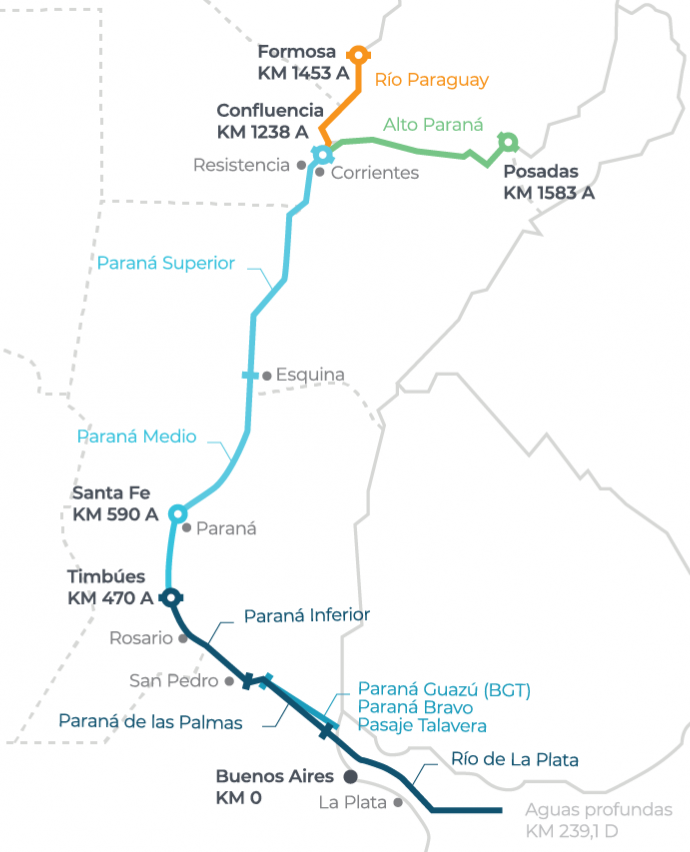
\includegraphics[width=0.5\linewidth]{figures/2025_mapa_vnt_extendida_tramos_profundidades_abril.png}
    \caption{The Vía Navegable Troncal (VNT) and the location of the Paraná Guazú in it \autocite{NavegableTroncal2025}}
    \label{fig:VNT}
\end{figure}

\section{Classification of Rio Paraná}

Rivers can be described and classified in different ways. This classification can be linked to several factors such as age, colour or seasonality. 

\subsection{The Age Classification of a River}
Based on the development of the channel stage of a river, it can be labeled as youthful, mature or old age.  \autocite{davisGeographicalCycle1899}
Applying this to the Rio Paraná makes it a complicated choice since the river is so long that it possesses features linked to each age label at distinct locations. therefore, it would be wiser to divide the Rio Paraná in three parts: upper, middle and lower Paraná. A youthful channel can be recognized through rapid flow, significant erosion, and a steep gradient. All these traits can be attributed to the upper Paraná zone.
Moving on, a mature channel stage of river is in most cases a developed floodplain in the form of loops, called 'meander', and lateral erosion. This is mostly what can be seen in the middle part of the Paraná river.
Lastly, the characteristics of an old age channel are comparable to the lower Paraná river. A wider floodplain, less rapid flow, and Deltas. All of this is explained in \autocite{orfeoParanaRiverArgentine2023}, and can be seen in the following figure from \autocite{lopezweibelSourcesTemporalDynamics2022}.



\begin{figure}[H]
    \centering    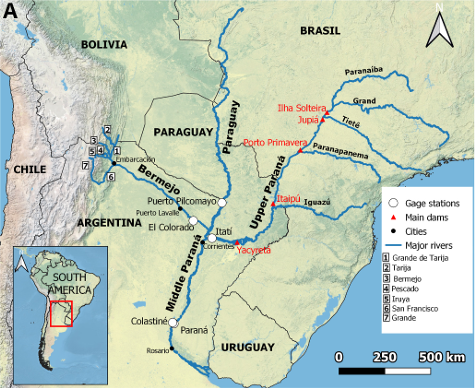
\includegraphics[width=0.5\linewidth]{figures/figure chap 2/map rio parana.png}
    \caption{Rio Paraná Map}
    \label{fig:placeholder}
\end{figure}


From Davis's study it makes sense that all these stages are represented in the total picture of the Paraná river since it is the ninth largest river in the world based on discharge \autocite{lopezweibelSourcesTemporalDynamics2022}.

\subsection{The Colour Classification of a River}
The colour of the river is also another label that can create a distinction. Based on two sets of papers/research  \autocite{furchWaterChemistryAmazon1984}, \autocite{sioliAmazonLimnologyLandscape1984}  Junk 1997, the water in rivers can be described as black, white or clear. The black water river is attributed to the 'leaching of tannins from decayed leaves of adjoining vegetated lands' \autocite{sand-mining-boek}, most comon in Amazonia or in the United States. White waters on the other hand are, contrary to its qualification, usually brown coloured due to the high sediment concentration. Clear water rivers are located in environments with little to no erosion.
Based on the theory and satellite imagery, one can again classify the Rio Paraná in different as a black and white river depending on the zone. The upper Paraná can be considered to be black due to its lack of sediment content, but rich in leaves content. But after the Bermejo river joins the Paraná, the river turns muddy all the way to the sea near Buenos Aires. \autocite{lopezweibelSourcesTemporalDynamics2022}

\begin{figure}[htbp]
    \centering
    \begin{subfigure}[b]{0.48\textwidth}
        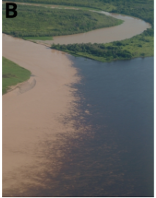
\includegraphics[width=\linewidth, height=5cm]{figures/figure chap 2/Paraguay-Bermejo.png}
        \caption{Confluence of the Paraguay and Bermejo River}
        \label{fig:bermejo}
    \end{subfigure}
    \hfill
    \begin{subfigure}[b]{0.48\textwidth}
        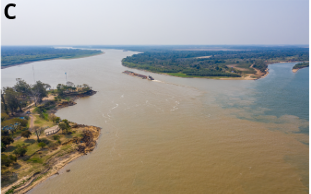
\includegraphics[width=\linewidth, height=5cm]{figures/figure chap 2/Paraguay Parana.png}
        \caption{Confluence of the Paraguay and Paraná River}
        \label{fig:parana}
    \end{subfigure}
    \caption{Confluences of the Paraguay River with the Bermejo (left) and Paraná (right)}
    \label{fig:confluences}
\end{figure}

\subsection{The Seasonal Flow of a River}
The last classification relevant for this study is based on the flow characteristics and water availability. There are once again three types of categories: ephemeral, intermediate and perennial rivers. Ephemeral means that the river flow is not continuously present throughout the calendar year. Perennial rivers are the rivers whose flow is continuous and does not dry up during dry season, unlike the ephemeral rivers. Lastly the intermediate rivers are perennial rivers that dry up in extreme cases of drought.
The Rio Paraná can be considered a perennial river due to its continuous flow over the years \autocite{furchWaterChemistryAmazon1984}, \autocite{sioliAmazonLimnologyLandscape1984}.
 
\section{Mining of the Sand and Types of Dredging in a River}
Due to the need of sand in our society, various techniques have been established to get hold of the sand in the river beds. In this subpart the different dredging techniques will be explained.
For the sake of this study the focus will lie on in stream mining, the extraction of sand and gravel from the active channel of a river \autocite{sand-mining-boek}.

\textit{Bar scalping or skimming}:
This is the most common practice of extraction. It consists of taking away the two thirds of the bar, leaving the top third to minimize the alternation of the river bed initial conditions.

\textit{Dry pit channel mining}:
This method relies on using tools (mechanical or manual) to create a dry pit in which the sand or gravel can be extracted. The state in which the pits are left after extraction act has head cuts, altering the upstream flow during the high seasons.

\textit{Wet pit channel mining}:
Usually, the pit is made in a perennial river, but the effects and damages are the same as for the dry pit channel mining.

\textit{Bar excavation}:
This excavation process happens downstream of the bar, in order to get a hold of the sand and gravel going downstream.

\textit{Instream traps}:
For this excavation method a hole is dug so that the sediment gets caught during high season. This sediment can later be captured when the tides are low again.



\section{The effects of river sand mining}
\subsection{River bed}
As mentioned in the previous section, rivers maintain an equilibrium between erosion, transport, and deposition of sediments. However, instream sand mining can discrupt this balance. This happens through direct disruption of the channel geometry or through so-called incision and related undercutting of banks \autocite{sand-mining-boek}.

The direct disruption of the river bed depends on the type of sand mining technique employed. In the case of pit excavation, the river bed is locally lowered and a so-called 'nick point' is created. With bar skimming the river bed is widened \autocite{sand-mining-boek}. For the remainder of this section, the consequent effects of the local river bed lowering (the nick point) are discussed.

Channel incision causes the nick point to migrate both upstream and downstream. In the case of high flows, due to its shape, the nick point is the point where most erosion occurs. Water plunges over the step and erodes the bed at the base. As flows continue, the drop migrates upstream, a process which is often called head-cutting in literature. On the other hand, a process called 'hungry water' causes downstream migration of the pit \autocite{sand-mining-boek}.

A the mining pit the water level is deeper, which causes the flow velocity to reduce locally. This leads to a decrease in flow energy and thus to more deposited sediment. When the flow leaves the mining area, water levels are shallower again meaning that flow velocity and energy significantly increase. A lot of sediment has been deposited in the nick point, meaning that the water is not using its full sediment carrying capacity anymore. In other words, the water is 'hungry' for sediment and erosion downstream increases \autocite{sand-mining-boek}. 

Through the combined effects of head-cutting and hungry water, the mining pit can extend beyond the initial dimensions caused by direct disruption. This happens in both downstream and upstream directions, as summarized in figure \ref{fig:channelbedeffects}.

\begin{figure}[H]
    \centering
    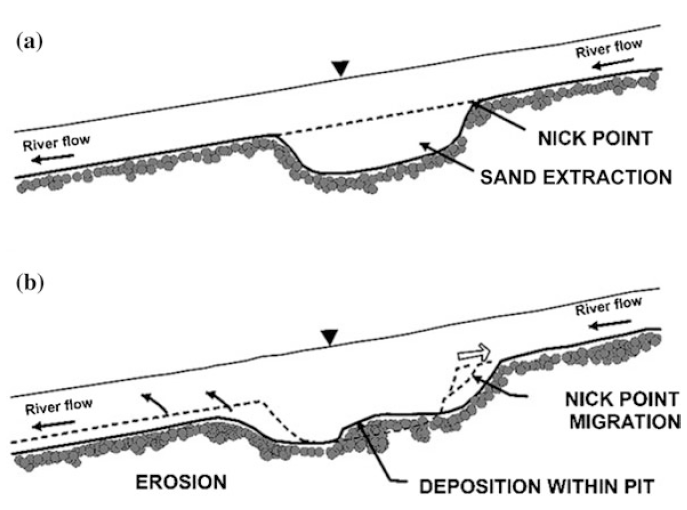
\includegraphics[width=0.75\linewidth]{figures/channelbedeffects.png}
    \caption{a: direct disruption leads to a locally lowered water bed, b: channel incision makes the pit migrate upstream through head cutting and downstream through 'hungry' water \autocite{sand-mining-boek}}
    \label{fig:channelbedeffects}
\end{figure}

\subsection{Sediment}
Previous studies have shown that bed coarsening can occur as a result of sand-mining. Fine particles are removed, leading to a greater concentration of coarse (gravelly) particles. This effect can also be seen upstream \autocite{sand-mining-boek}.

\subsection{Water quality and quantity}
Sand mining can lead to changes in both water quality and quantity. The process of dredging the fine sand stirs fine organic and inorganic particles, thereby increasing the turbidity of the water. This reduces light penetration, which means less photosynthesis and ultimately less organic growth in the water \autocite{sharipEffectsSeasonSand2014}.

As mentioned before, mining pits are often places with significant deposition of particles. Fine, nutrient-rich particles can settle and get trapped in the pits. This then reduces the transport of nutrients from the river to the coastal waters \autocite{sand-mining-boek}.

Concerning the water quantity, the most relevant effects are related to the groundwater: the lowering of the river bed through direct disruption or channel incision can lead to a lower groundwater table. This can lead to settlements or have negative effects on flora and fauna surrounding the river \autocite{rentierEnvironmentalImpactsRiver2022}.

\subsection{Biologic, socioeconomic and infrastructural changes}
The effects of sand mining can be diverse: previous studies have shown negative impacts on biodiversity, including reduced benthic fauna, disrupted fish spawning habitats, and depletion of natural mosquito predators such as dragonflies \autocite{sand-mining-boek}. The socioeconomic effects of mining can vary, in the short-term it often provides employment, income, and government revenue through royalties and taxation. However, in the long-term the operation can cause a reduction in access to clean water and can cause water scracity, especially in dry periods. Additionally, loss of land and access to land together with loss of trees and vegetation can jeapordize the local food security. Finally, infrastructure can be damaged by the lowering of the river bed and/or the groundwater table \autocite{sand-mining-boek}.


\section{Origin of sediment content in Paraná Guazú}

A key step in constructing the sediment balance of the Paraná Guazú, located in the lower Paraná, is to identify the origin of its sediment. As shown in Figure \ref{fig:placeholder}, the lower and middle Paraná receive discharge from three main tributaries: the Bermejo, Paraguay, and upper Paraná rivers. The total average discharge in the middle Paraná is $18,389~\mathrm{m^3/s}$, of which 78\% is supplied by the upper Paraná. \citeauthor{lopezweibelSourcesTemporalDynamics2022} report that the Bermejo contributes only 2\% of this discharge. Nevertheless, the Bermejo is the dominant source of sediment, due to intense erosion in the Andes Eastern Mountain Range within its basin. During the wet season (November to April), multiple tributaries in the basin contribute large sediment flows, accumulating to an annual suspended sediment load of $106 ~\times 10^6$ t per year at El Colorado gauge station. By contrast, sediment supply from the upper Paraná is strongly reduced by hydropower dams that trap material upstream. 

It is interesting to know that the contribution of sediment from the Bermejo to the Paraná is approximately 90\% today, but that this is in fact due to the installation of the Itaipu dam built in 1971. This modification of the sediment voyage cuts a supply of about 50\% compared the initial amount of sediment, this 90\% used to be 56\% of the sediment income before the construction of the dam. This explains us that the involvement of the 

In summary, while the Paraguay and upper Paraná rivers provide most of the fluvial discharge to the downstream delta, the Bermejo River delivers the majority of sediments (\cite{lopezweibelSourcesTemporalDynamics2022}). For this reason, the stretch of river beginning in the Bermejo basin and continuing via the Paraguay and middle Paraná to the Paraná Guazú is of particular importance in this study.  













\chapter{Background Study}
In this part of the report, the research that contributes to the contextualization of the Rio Paraná Guazú will be explained. The goal of the background study is to give the lector an understanding of what theory is used for the later stages of the analysis.

\section{Argentina's waterways}
The Argentine river system can be grouped into three watersheds: the Atlantic watershed, which drain into the Argentine Sea, the Pacific watershed; and, finally the rivers that don't drain into an ocean but flow inland to permanent or seasonal lakes, swamps, or dry sinks. Of these systems, the Atlantic watershed is the most important and includes the Río de la Plata Basin, the Patagonian system, and several smaller rivers in the province of Buenos Aires \autocite{marioe.farberHydrographyArgentina2024}. The Río de la Plata Basin is the most relevant one: it ends in the Río de la Plata estuary and consists of the Paraná, the country's longest river, the Uruguay and their subrivers. The Vía Navegable Troncal (VNT) ends in the Río de la Plata estuary and connects numerous ports to the ocean. Because of this, the VNT is responsible for rougly 80\% of the nation's export \autocite{NavegableTroncal2025}. The Paraná Guazú is part of this main waterway, as can be seen in figure \ref{fig:VNT}.

\begin{figure}
    \centering
    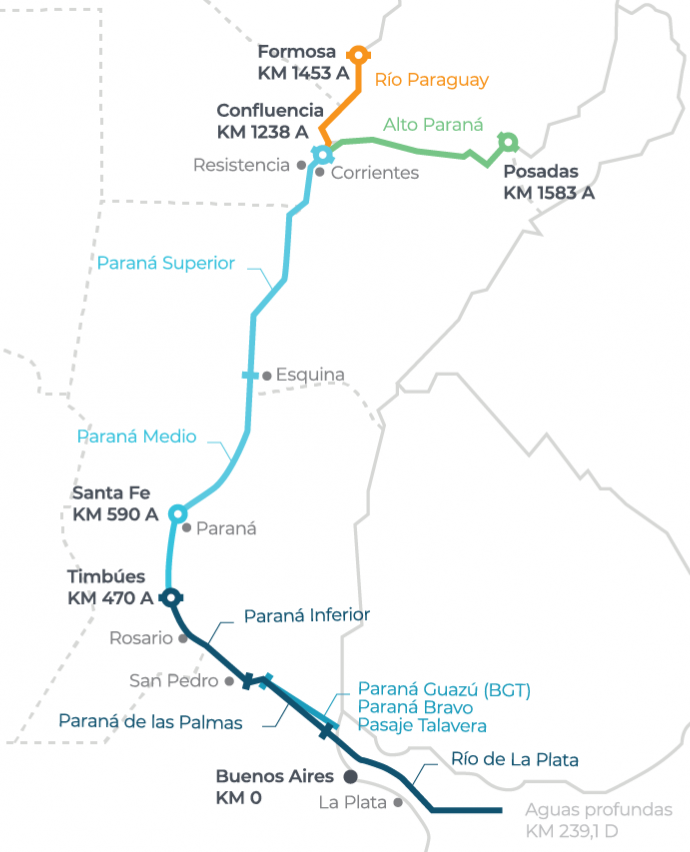
\includegraphics[width=0.5\linewidth]{figures/2025_mapa_vnt_extendida_tramos_profundidades_abril.png}
    \caption{The Vía Navegable Troncal (VNT) and the location of the Paraná Guazú in it \autocite{NavegableTroncal2025}}
    \label{fig:VNT}
\end{figure}

\section{Classification of Rio Paraná}

Rivers can be described and classified in different ways. This classification can be linked to several factors such as age, colour or seasonality. 

\subsection{The Age Classification of a River}
Based on the development of the channel stage of a river, it can be labeled as youthful, mature or old age.  \autocite{davisGeographicalCycle1899}
Applying this to the Rio Paraná makes it a complicated choice since the river is so long that it possesses features linked to each age label at distinct locations. therefore, it would be wiser to divide the Rio Paraná in three parts: upper, middle and lower Paraña. A youthful channel can be recognized through rapid flow, significant erosion, and a steep gradient. All these traits can be attributed to the upper Paraná zone.
Moving on, a mature channel stage of river is in most cases a developed floodplain in the form of loops, called 'meander', and lateral erosion. This is mostly what can be seen in the middle part of the Paraná river.
Lastly, the characteristics of an old age channel are comparable to the lower Paraná river. A wider floodplain, less rapid flow, and Deltas. All of this is explained in \autocite{orfeoParanaRiverArgentine2023}, and can be seen in the following figure from \autocite{lopezweibelSourcesTemporalDynamics2022}.



\begin{figure}[H]
    \centering    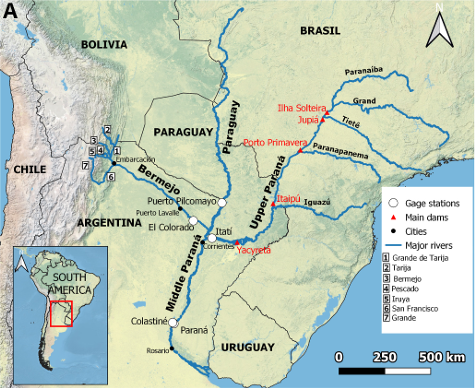
\includegraphics[width=0.5\linewidth]{figures/figure chap 2/map rio parana.png}
    \caption{Rio Paraná Map}
    \label{fig:placeholder}
\end{figure}


From Davis's study it makes sense that all these stages are represented in the total picture of the Paraná river since it is the ninth largest river in the world based on discharge \autocite{lopezweibelSourcesTemporalDynamics2022}.

\subsection{The Colour Classification of a River}
The colour of the river is also another label that can create a distinction. Based on two sets of papers/research  \autocite{furchWaterChemistryAmazon1984}, \autocite{sioliAmazonLimnologyLandscape1984}  Junk 1997, the water in rivers can be described as black, white or clear. The black water river is attributed to the 'leaching of tannins from decayed leaves of adjoining vegetated lands' \autocite{sand-mining-boek}, most comon in Amazonia or in the United States. White waters on the other hand are, contrary to its qualification, usually brown coloured due to the high sediment concentration. Clear water rivers are located in environments with little to no erosion.
Based on the theory and satellite imagery, one can again classify the Rio Paraná in different as a black and white river depending on the zone. The upper Paraná can be considered to be black due to its lack of sediment content, but rich in leaves content. But after the Bermejo river joins the Paraná, the river turns muddy all the way to the sea near Buenos Aires. \autocite{lopezweibelSourcesTemporalDynamics2022}

\begin{figure}[htbp]
    \centering
    \begin{subfigure}[b]{0.48\textwidth}
        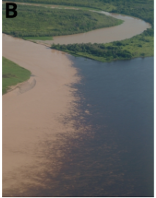
\includegraphics[width=\linewidth, height=5cm]{figures/figure chap 2/Paraguay-Bermejo.png}
        \caption{Confluence of the Paraguay and Bermejo River}
        \label{fig:bermejo}
    \end{subfigure}
    \hfill
    \begin{subfigure}[b]{0.48\textwidth}
        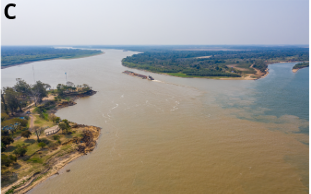
\includegraphics[width=\linewidth, height=5cm]{figures/figure chap 2/Paraguay Parana.png}
        \caption{Confluence of the Paraguay and Paraná River}
        \label{fig:parana}
    \end{subfigure}
    \caption{Confluences of the Paraguay River with the Bermejo (left) and Paraná (right)}
    \label{fig:confluences}
\end{figure}

\subsection{The Seasonal Flow of a River}
The last classification relevant for this study is based on the flow characteristics and water availability. There are once again three types of categories: ephemeral, intermediate and perennial rivers. Ephemeral means that the river flow is not continuously present throughout the calendar year. Perennial rivers are the rivers whose flow is continuous and does not dry up during dry season, unlike the ephemeral rivers. Lastly the intermediate rivers are perennial rivers that dry up in extreme cases of drought.
The Rio Paraná can be considered a perennial river due to its continuous flow over the years \autocite{furchWaterChemistryAmazon1984}, \autocite{sioliAmazonLimnologyLandscape1984}.
 
\section{Mining of the Sand and Types of Dredging in a River}
Due to the need of sand in our society, various techniques have been established to get hold of the sand in the river beds. In this subpart the different dredging techniques will be explained.
For the sake of this study the focus will lie on in stream mining, the extraction of sand and gravel from the active channel of a river \autocite{sand-mining-boek}.

\textit{Bar scalping or skimming}:
This is the most common practice of extraction. It consists of taking away the two thirds of the bar, leaving the top third to minimize the alternation of the river bed initial conditions.

\textit{Dry pit channel mining}:
This method relies on using tools (mechanical or manual) to create a dry pit in which the sand or gravel can be extracted. The state in which the pits are left after extraction act has head cuts, altering the upstream flow during the high seasons.

\textit{Wet pit channel mining}:
Usually, the pit is made in a perennial river, but the effects and damages are the same as for the dry pit channel mining.

\textit{Bar excavation}:
This excavation process happens downstream of the bar, in order to get a hold of the sand and gravel going downstream.

\textit{Instream traps}:
For this excavation method a hole is dug so that the sediment gets caught during high season. This sediment can later be captured when the tides are low again.



\section{The effects of river sand mining}
\subsection{River bed}
As mentioned in the previous section, rivers maintain an equilibrium between erosion, transport, and deposition of sediments. However, instream sand mining can discrupt this balance. This happens through direct disruption of the channel geometry or through so-called incision and related undercutting of banks \autocite{sand-mining-boek}.

The direct disruption of the river bed depends on the type of sand mining technique employed. In the case of pit excavation, the river bed is locally lowered and a so-called 'nick point' is created. With bar skimming the river bed is widened \autocite{sand-mining-boek}. For the remainder of this section, the consequent effects of the local river bed lowering (the nick point) are discussed.

Channel incision causes the nick point to migrate both upstream and downstream. In the case of high flows, due to its shape, the nick point is the point where most erosion occurs. Water plunges over the step and erodes the bed at the base. As flows continue, the drop migrates upstream, a process which is often called head-cutting in literature. On the other hand, a process called 'hungry water' causes downstream migration of the pit \autocite{sand-mining-boek}.

A the mining pit the water level is deeper, which causes the flow velocity to reduce locally. This leads to a decrease in flow energy and thus to more deposited sediment. When the flow leaves the mining area, water levels are shallower again meaning that flow velocity and energy significantly increase. A lot of sediment has been deposited in the nick point, meaning that the water is not using its full sediment carrying capacity anymore. In other words, the water is 'hungry' for sediment and erosion downstream increases \autocite{sand-mining-boek}. 

Through the combined effects of head-cutting and hungry water, the mining pit can extend beyond the initial dimensions caused by direct disruption. This happens in both downstream and upstream directions, as summarized in figure \ref{fig:channelbedeffects}.

\begin{figure}[H]
    \centering
    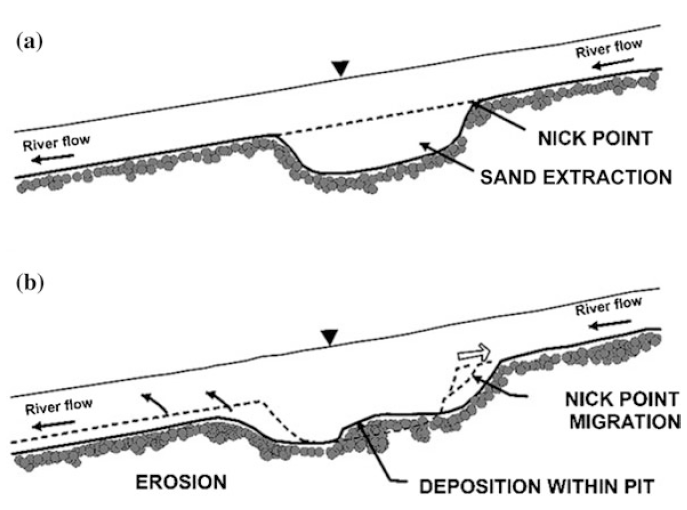
\includegraphics[width=0.75\linewidth]{figures/channelbedeffects.png}
    \caption{a: direct disruption leads to a locally lowered water bed, b: channel incision makes the pit migrate upstream through head cutting and downstream through 'hungry' water \autocite{sand-mining-boek}}
    \label{fig:channelbedeffects}
\end{figure}

\subsection{Sediment}
Previous studies have shown that bed coarsening can occur as a result of sand-mining. Fine particles are removed, leading to a greater concentration of coarse (gravelly) particles. This effect can also be seen upstream \autocite{sand-mining-boek}.

\subsection{Water quality and quantity}
Sand mining can lead to changes in both water quality and quantity. The process of dredging the fine sand stirs fine organic and inorganic particles, thereby increasing the turbidity of the water. This reduces light penetration, which means less photosynthesis and ultimately less organic growth in the water \autocite{sharipEffectsSeasonSand2014}.

As mentioned before, mining pits are often places with significant deposition of particles. Fine, nutrient-rich particles can settle and get trapped in the pits. This then reduces the transport of nutrients from the river to the coastal waters \autocite{sand-mining-boek}.

Concerning the water quantity, the most relevant effects are related to the groundwater: the lowering of the river bed through direct disruption or channel incision can lead to a lower groundwater table. This can lead to settlements or have negative effects on flora and fauna surrounding the river \autocite{rentierEnvironmentalImpactsRiver2022}.

\subsection{Biologic, socioeconomic and infrastructural changes}
The effects of sand mining can be diverse: previous studies have shown negative impacts on biodiversity, including reduced benthic fauna, disrupted fish spawning habitats, and depletion of natural mosquito predators such as dragonflies \autocite{sand-mining-boek}. The socioeconomic effects of mining can vary, in the short-term it often provides employment, income, and government revenue through royalties and taxation. However, in the long-term the operation can cause a reduction in access to clean water and can cause water scracity, especially in dry periods. Additionally, loss of land and access to land together with loss of trees and vegetation can jeapordize the local food security. Finally, infrastructure can be damaged by the lowering of the river bed and/or the groundwater table \autocite{sand-mining-boek}.


\section{Origin of sediment content in Paraná Guazú}

A key step in constructing the sediment balance of the Paraná Guazú, located in the lower Paraná, is to identify the origin of its sediment. As shown in Figure \ref{fig:placeholder}, the lower and middle Paraná receive discharge from three main tributaries: the Bermejo, Paraguay, and upper Paraná rivers. The total average discharge in the middle Paraná is $18,389~\mathrm{m^3/s}$, of which 78\% is supplied by the upper Paraná. \citeauthor{lopezweibelSourcesTemporalDynamics2022} report that the Bermejo contributes only 2\% of this discharge. Nevertheless, the Bermejo is the dominant source of sediment, due to intense erosion in the Andes Eastern Mountain Range within its basin. During the wet season (November to April), multiple tributaries in the basin contribute large sediment flows, accumulating to an annual suspended sediment load of $106 ~\times 10^6$ t per year at El Colorado gauge station. By contrast, sediment supply from the upper Paraná is strongly reduced by hydropower dams that trap material upstream.  

In summary, while the Paraguay and upper Paraná rivers provide most of the fluvial discharge to the downstream delta, the Bermejo River delivers the majority of sediments (\cite{lopezweibelSourcesTemporalDynamics2022}). For this reason, the stretch of river beginning in the Bermejo basin and continuing via the Paraguay and middle Paraná to the Paraná Guazú is of particular importance in this study.  













\chapter{Stakeholder analysis}
\label{chapter:stakeholders}

In this part of the report, the stakeholders related to Rio Paraná Guazú will be explained. The goal of this stakeholder analysis is to understand the different interests in the region related to sand dredging activities.


\section{Stakeholders}

For the stakeholder analysis, all potentially relevant stakeholders for this project were identified. Some were suggested directly by INA staff, who indicated individuals important for gathering information on the Parana Guazú River. Additional stakeholders were identified through further investigation into relevant contacts. The full list of these stakeholders appears in Table \ref{tab:stakeholders} and will be discussed in the following sections.

\subsubsection{Stakeholders}

\begin{table}[ht]
\centering
\begin{tabularx}{\linewidth}{lX}
\toprule
\textbf{Stakeholder} & \textbf{Role} \\
\midrule
Dredgers & Extraction of sand \\
\midrule
Dredging Companies & Extraction and selling of sand \\
\midrule
Prefectura Naval Argentina & Protects rivers and maritime territory \\
\midrule
Agencia Nacional de Puertos y Navegación & Control of signalling system, dredging, and maintenance \\
\midrule
Ports & Handling and storing of goods \\
\midrule
Fishermen & Local fishermen \\
\midrule
NGOs & Non-profit organizations \\
\midrule
Agua y Saneamientos Argentinos & Delivering water and sewerage services \\
\midrule
Alejo Di Rosio & Filmmaker \\
\bottomrule
\end{tabularx}
\caption{Potential stakeholders}
\label{tab:stakeholders}
\end{table}

\subsubsection{Stakeholders description}

The stakeholders which where given in the overview here above will be shortly described in the following overview. Hereafter, the stakheolders will be described in more detail to get a better understanding of the interests and goals of each specific stakeholder. In Table X an overview of the descriptions is given.

\begin{table}[ht]
\centering
\begin{tabularx}{\linewidth}{lX}
\toprule
\textbf{Stakeholder} & \textbf{Description} \\
\midrule
Dredgers & Extraction of sand \\
\midrule
Dredging Companies & Extraction and selling of sand \\
\midrule
Prefectura Naval Argentina & Protects rivers and maritime territory \\
\midrule
Agencia Nacional de Puertos y Navegación & Control of signalling system, dredging, and maintenance \\
\midrule
Ports & Handling and storing of goods \\
\midrule
Fishermen & Local fishermen \\
\midrule
NGOs & Non-profit organizations \\
\midrule
Agua y Saneamientos Argentinos & Delivering water and sewerage services \\
\midrule
Alejo Di Rosio & Filmmaker \\
\bottomrule
\end{tabularx}
\caption{Potential stakeholders with descriptions}
\label{tab:stakeholders-description}
\end{table}




\subsubsection{Stakeholder interests, problem perception and goal}



\section{Dredgers (LOCAL??)}
The first dominant group of stakeholders are the dredgers.These include the local boats used in the area to extract sand and gravel from the river. There are several different types of dredgers ranging from small independent boats, to groups of small boats that work for the same employer (ARENEROS??), or big extracting ships commonly referred to as 'hoppers'. In the area of interest, the Paraná Guazú from Ibicuy to Brazo Largo, the most common dredgers are: (ARENEROS, INDEPENDENT BOATS). 

Currently there are 2 active boats in the zone of the Rio Paraná Guazú of interest, and (QUITE A LOT MORE IN IBICUY?? FROM INTERVIEW), as mentioned in the previous Chapter. (DREDGING ACTIVITY AANGEVEN WELKE BOTEN, MAPS MET HEEN EN TERUG REIS, DATA , ETC)

Their interest in the Rio Paraná Guazú is to extract the sand in locations of the river that are shallow since they do not possess any technology to mine the sand from deep. Once this water mixed sand is lifted onto the boat, they transport it to the nearest ports, Ibicuy or Brazo Largo. They sell their sand to the highest bidder which can be for (PURPOSES FROM INTERVIEW).


\section{BIG Dredging Companies?}
because they buy the sand and employ the areneros?
The Dredging companies active in the Rio Paraná Guazú are :
(EERST KIJKEN OF YPF, JAn de NUl, etc hierbij kan worden betrokken of niet)


\section{Prefectura Naval Argentina}
The Prefectura Naval Argentina (PNA), is the National Naval Prefecture of the Rio Paraná. Therefore, they are also active in the Paraná Guazú and our area of surveillance. 
It is in their interest to protect the Rio Paraná Guazú from criminal activities. These can 

\section{Agencia Nacional de Puertos y Navegación}
The Agencia Nacional de Puertos y Navegación (ANPYN), or the National Agency of Ports and Navigation, was created on January 6, 2025 by a merger of the Undersecretariat of Ports, Waterways and Merchant Marine and the General Port Administration. Since then, the agency has taken over the tasks of the two former entities and is now responsible for policies concerning ports, waterways and river and maritime transport. As such, keeping the Vía Navegable Troncal (VNT), Argentina's main waterway, navigable for ships is an important task for the agency. To achieve this, they regulate dredging and sand mining contracts and oversee compliance with the relevant regulations .

\section{Ports}
In the researched area there are two strategic port locations that play a key role in the sand extraction.

\subsection{Guazú}
?
\subsection{Ibicuy}
?

\section{Fishermen}
Fischermen is another stakeholder group relevant for this study. The Rio Paraná Guazu is used by a lot of people for its high concentration of fish. 

The artisanal fisheries play an economic role as most of the harvest is sold to middlemen, freezing plants, or in informal markets. Of particular interest are long-range migratory species such as sábalo (Prochilodus lineatus), surubí (Pseudoplatystom corruscans, P. reticulatus), boga (Megaleporinus obtusidens), pacú (Piaractus mesopotamicus), and dorado (Salminus brasiliensis), that support artisanal, recreational, and subsistence fisheries, as observed in other large neotropical rivers, \autocite{assessment of sabalo}, \autocite{fishers' knowledge}

the fischermen in the region of interest are mostly independent. Even though there exists such thing as fischermen associations in the Rio Paraná Guazú, they are not influencial 



\section{NGO's}
even wachten tot ik een nice milieu organisatie vind.

\section{Agua y Saneamientos Argentinos}
Even wachten tot interview met hun, kijken of ze wel relevant zijn


\section{Filmmaker}

When researching for the stakeholders which were relevant for the analysis. We stumble upon an article on a film that was made on the Parana-Paraguay waterway. In this documentary, the focus is on the impact of the trade happening on the Parana-Paraguay waterway. The documentary is made by filmmaker Alejo Di Risio, who was contacted through journalist Matias Avramow for any additional information about stakeholders and business related to the waterway.


\chapter{Data Analysis}

\section{Dredging activity}
This section describes the relevance of dredging to the sediment balance of the designated area, by an estimation of the dredging volumes through different data sources. It includes an analysis of the data gathered through AIS and extraction permits. 


\subsection{Vessel positioning information (AIS)}

Using MarineTraffic it was found that two dredgers are operating on the Paraná Guazú between Ibicuy and Brazo Largo: the Comercio Segundo and the E.M. Arroyo N1. The Comercio Segundo has a length of 30 m, a width of 7 m, a draft of 1.3 m, and an approximate cargo hold of 195 m\textsuperscript{3}. The E.M. Arroyo N1 has a length of 39 m, a width of 8 m, a draught of 2.8 m and an approximate cargo hold of 476 \,m\textsuperscript{3}. Using a sand to water ratio of 3:1 for the dredged slurry, the amount of sand dredged is 150 \,m\textsuperscript{3} and 360 \,m\textsuperscript{3} respectively per cargo. The tracks of the two vessels obtained from MarineTraffic are shown in Figures 5.1 and 5.2.

\begin{figure}[h!]
    \centering
    \begin{minipage}{0.48\textwidth}
        \centering
        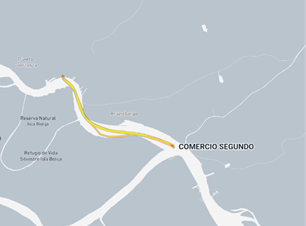
\includegraphics[width=\linewidth]{figures/ch5/Track_CS.png}
        \caption{Track of the \textit{Comercio Segundo}}
        \label{fig:track_cs}
    \end{minipage}\hfill
    \begin{minipage}{0.48\textwidth}
        \centering
        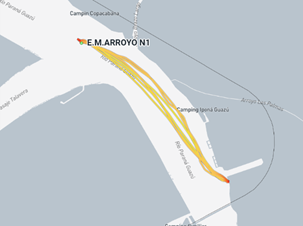
\includegraphics[width=\linewidth]{figures/ch5/Track_EM.png}
        \caption{Track of the \textit{E.M. Arroyo N1}}
        \label{fig:track_em}
    \end{minipage}
\end{figure}

The AIS data for these two vessels is obtained from MyShipTracking, which is used to determine the location of the dredging and the average number of trips. The dredging location of the two vessels is shown in Figure 5.3. It can be seen that both dredgers dredge in the same area. This can be explained by the bathymetry shown in Figure 5.4, which shows a reduced depth near the junction of the two navigable channels. At this location the flow velocity is lower, causing sediment to settle and thus creating a sandbar. From the AIS data it can be concluded that both dredgers make three trips per day.

\begin{figure}[h!]
    \centering
    \begin{minipage}{0.48\textwidth}
        \centering
        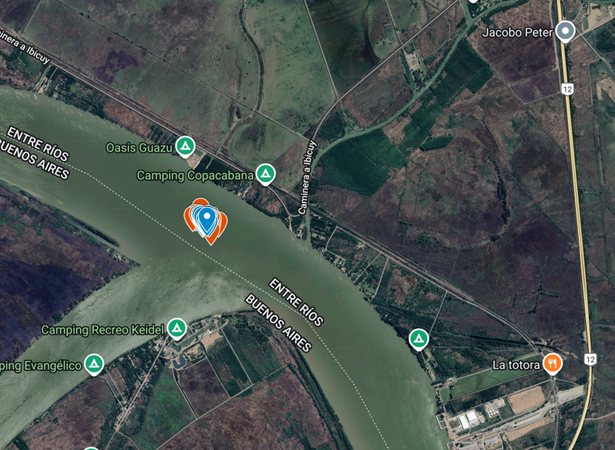
\includegraphics[width=\linewidth]{figures/ch5/Dredging_coordinates.png}
        \caption{Dredging location}
        \label{fig:dredging_coordinates}
    \end{minipage}\hfill
    \begin{minipage}{0.48\textwidth}
        \centering
        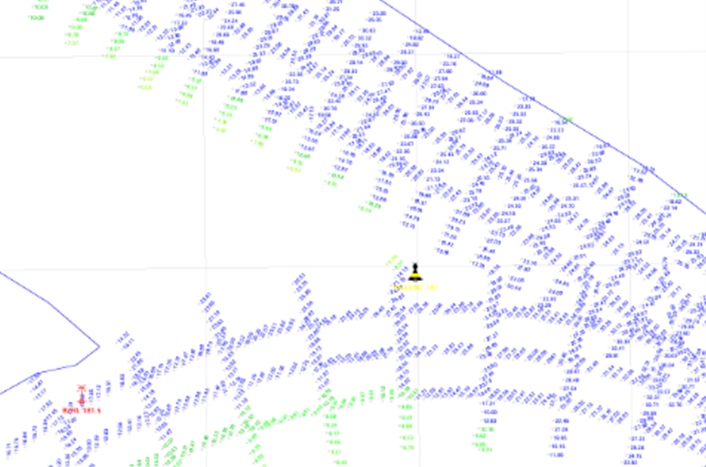
\includegraphics[width=\linewidth]{figures/ch5/Bathymetry.png}
        \caption{Bathymetry}
        \label{fig:bathymetry}
    \end{minipage}
\end{figure}

In the Rio Talabera, a side branch connecting to the Paraná Guazú, a third dredger is extracting sand. The Altair is dredger with a length of 66 m, a width of 11 m, a draught of 1.5 m and a approximate cargo hold of 750 \,m\textsuperscript{3}. Using the same sand to water ratio of 3:1 this gives 560 \,m\textsuperscript{3} of sand per cargo. Using MarineTraffic it was found that the Altair has an average 3 trips per day. Figure 5.5 shows the track of the Altair and the location at which it stops to extract sand. 

\begin{figure}[H]
    \centering
    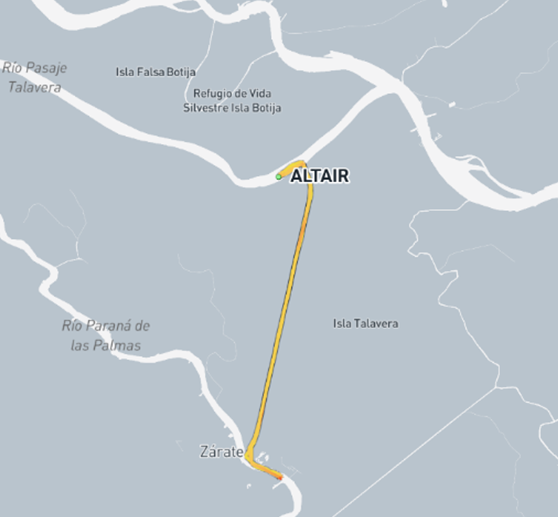
\includegraphics[width=0.5\linewidth]{figures/ch5/Track_Altair.png}
    \caption{Track of the Altair}
    \label{fig:placeholder}
\end{figure}

For all three vessels, the estimated volume of sand extracted per month is displayed in table 5.1
\begin{table}[h!]
\centering
\begin{tabular}{lrrrr}
\hline
\textbf{Vessel} & \textbf{Cargo hold} & \textbf{Sand volume [\,m\textsuperscript{3}]} & \textbf{Trips per day} & \textbf{Volume per month [\,m\textsuperscript{3}]} \\
\hline
Comercio Segundo & 195 & 150 & 3 & 9000 \\
E.M. Arroyo N1 & 476 & 360 & 3 & 21600 \\
Altair & 750 & 560 & 3 & 33600 \\
\hline
\end{tabular}
\caption{Sand transport details per vessel.}
\label{tab:sand_volume}
\end{table}


\subsection{Extraction permits}
A total of 33 permits were collected for the Paraná Guazú and 43 for the Ibicuy. On the Paraná Guazú, four permits were issued for channel maintenance, while the remainder concerned sand extraction. For the Ibicuy, all permits were related to extraction activities. The analysis shows that the requested volumes in the Ibicuy are considerably larger than those in the Paraná Guazú, even though the section of the Ibicuy considered here is much shorter in length.

It is important to note that the end dates of contracts are unknown. While the requests specify monthly dredging quantities, they do not indicate the duration of the works. As a result, a detailed quantitative assessment cannot be made. For the present analysis, all requests with fixed monthly volumes are assumed to extend over 12 months, allowing for a comparison between the two river sections, as shown in Figure \ref{fig:yearly dredging volumes}. The second assumption is to record a single value for the requested volume, when information about monthly or yearly occurrence is lacking.

\begin{figure}[H]
    \centering
    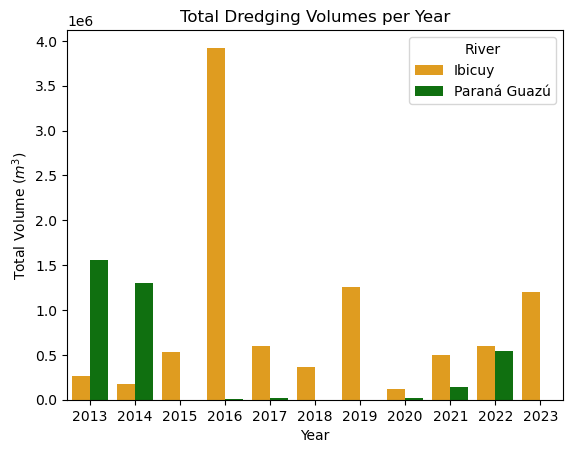
\includegraphics[width=0.50\linewidth]{figures/ch2/Dredging volumes permits.png}
    \caption{Yearly dredging volumes}
    \label{fig:yearly dredging volumes}
\end{figure}

\subsection{Estimated sand extraction}
This section draws a conclusion on the sand extraction volumes, such that an estimate is found to apply in the sediment balance. The following uncertainties were considered in determining a representative value:

\begin{itemize}
    \item Not every vessel in the area is equipped with an AIS transponder, meaning that possibly not all active vessels were identified
    \item No historical AIS data was available, such that the data was registered for only a short period of time 
    \item The extraction permits do not mention the duration of the contract
\end{itemize}

However, a rough estimate can be found by calculating the mean annual volume for the total system of interest (i.e., Ibicuy and Paraná Guazú). To make a comparison with the monthly values in Table \ref{tab:sand_volume}, this yearly value is reduced to a monthly value by dividing by 12 months. The former approach yields the following value for dredged sand volumes:

\begin{equation}
    V_{sand,yearly} = 1193923 ~m^3
\end{equation}
\begin{equation}
    V_{sand,monthly} = \frac{V_{sand,yearly}}{12} \approx 100000 ~m^3 
\end{equation}


\section{Hydrodynamic data}
nog introductie toevoegen

\\ \textbf{Tidal forcing}
\\The tidal wave of the Atlantic Ocean influences the hydrodynamics of the lower Paraná delta. As the tidal wave enters the delta ta Río de la Plata, the tide is damped and phased by friction, channel geometry and branching, resulting in a reduced amplitude and an increased in phase delay. Under normal conditions, the influence of the tide on the Paraná River reaches the city of Villa Constitución, which is located 220 km upstream of the river mouth. For storm conditions, the tide can reach the city of Rosario \autocite{balayCAUSESPERIODICITYLARGE}. In order to determine the influence of the tide at Brazo Largo, a reference water level at San Fernando is considered. It is assumed that at San Fernando no tidal damping has occurred, therefore the tidal amplitude at Brazo Largo can be determined using the following relation:

\begin{equation}
    A_{\text{Location}} = \alpha \cdot A_{\text{SanFernando}}
\end{equation}

The damping coefficient ($\alpha$) and the tidal delay with respect to San Fernando have been determined by Brok (2022). For Brazo Largo, a damping coefficient of 0.3 and tidal delay of 4 hours were found. These values will be used as reference values when isolating the tide at Brazo Largo. The tidal signal is isolated using hourly water level data for a period of more than 2 years from both Brazo Largo and San Fernando. Table 5.2 shows the tidal constituents  considered and their period.

\begin{table}[h!]
\centering
\caption{Tidal constituents used to reconstruct the tide
\autocite{BRON}.}
\label{tab:constituents}
\begin{tabular}{lccc}
\hline
\textbf{Tidal constituent} & \textbf{Name} & \textbf{Period [h]} \\
\hline
\multicolumn{3}{l}{\textit{Semi-diurnal}} \\
\hspace{1em}Principal lunar & M2 & 12.4206\\
\hspace{1em}Principal solar & S2 & 12.0000 \\
\hspace{1em}Lunar elliptical & N2 & 12.6583\\
\hline
\multicolumn{3}{l}{\textit{Diurnal}} \\
\hspace{1em}Lunar-solar declinational & K1 & 23.9345  \\
\hspace{1em}Principal lunar & O1 & 25.8193  \\
\hline
\multicolumn{3}{l}{\textit{Shallow water constituents}} \\
\hspace{1em}Overtide of M2 (quarter-diurnal) & M4 & 6.2103  \\
\hline
\end{tabular}
\end{table}

- uitleg hoe het getijde bepaald is

The tidal amplitude and phase of each constituent for San Fernando and Brazo Largo are displayed in Table 5.3. Additionally, the damping coefficient ($\alpha$) and the tide delay are calculated for the different constituents and shown in Table 5.3. The calculated amplitudes show that the delta has mixed tidal dynamics  (semidiurnal-diurnal)
dominated by the semi-diurnal M2 constituent with contributions from N2, K1 and O1. The overtide M4 plays a minor role. The damping coefficient is consistent across the constituents ranging from 0.23 to 0.33, inditcating that the use of formula 5.3 is valid. The calculated time delay of 4.5 - 5.5 hours is also in line with the time delay calculated by Brok (2022). The overtide M4 


\begin{table}[h!]
\centering
\caption{Amplitude and phase comparison}
\begin{tabular}{lcccccc}
\hline
Constituent & $A_{\text{SF}}$ & $A_{\text{BL}}$ & $\alpha$ & tide delay [hr] & $\phi_{\text{SF}}$ [$^\circ$] & $\phi_{\text{BL}}$ [$^\circ$] \\
\hline
M2 & 0.253 & 0.058 & 0.230 & 4.450 & -0.465 & 1.786 \\
S2 & 0.041 & 0.010 & 0.239 & 5.055 & -2.526 & 0.121 \\
N2 & 0.094 & 0.022 & 0.238 & 4.316 & -0.546 & 1.596 \\
K1 & 0.119 & 0.037 & 0.313 & 5.181 & -2.543 & -1.183 \\
O1 & 0.187 & 0.061 & 0.328 & 5.517 & 2.694 & -2.247 \\
M4 & 0.030 & 0.006 & 0.189 & -1.495 & -2.608 & 2.162 \\
\hline
\end{tabular}
\end{table}

Figure 5.7 shows the water level time series for a period of 7 days compared to the calculated tidal signal at Brazo Largo. From this figure, it can be seen that the measured water level follows the same tidal oscillations. However, the tide does not explain all the variability of the water level; the measured water level also shows large variability caused by discharge and wind. 
\\The influence of the strong non-tidal component is confirmed by Figure 5.8, which shows the water level at Brazo Largo for a period of 2 years. The measured water level fluctuates greatly, reaching +2.0 m and -0.5 m while the tidal component is steady at 0.0 m with an amplitude of 0.17 m. The tidal forcing is relatively small compared to the river and seasonal influences. Tidal forcing is therefore subordinate to other forcings such as discharge.

\begin{figure}[H]
    \centering
    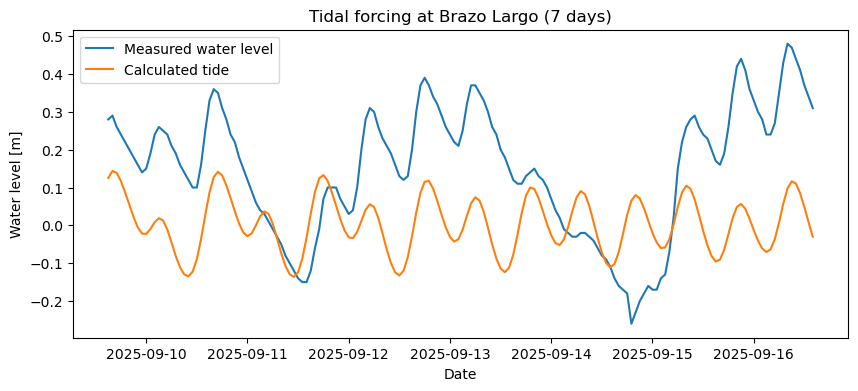
\includegraphics[width=1\linewidth]{figures/ch5/Tide_Brazo_largo.png}
    \caption{Calculated tide at Brazo Largo for a period of 7 days.}
    \label{fig:placeholder}
\end{figure}
\begin{figure}[H]
    \centering
    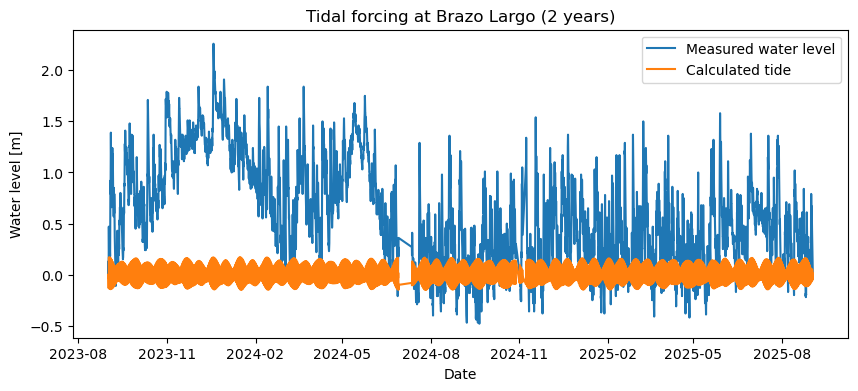
\includegraphics[width=1\linewidth]{figures/ch5/Tide_BL_2y.png}
    \caption{Calculated tide at Brazo Largo for a period of 2 years.}
    \label{fig:placeholder}
\end{figure}

\\- Waterlevel at Brazo Largo
    (misschien het getijde meenemen?)
\\ - Getijde rond Brazo Largo is berekend aan de hand van waterlevel rond San Fernando. Vergelijk de constituents met die van  het rapport en trek conclusie over invloed getijde.

\textbf{Fluvial forcing}

The relationship between fluvial discharge and water level at Brazo Largo was initially assumed to follow a power-law ($h = a \cdot Q^b$), but this yielded a weak correlation with an $R^2$ of 0.261. A linear fit, however, produced a slightly better result, showing a positive trend with an $R^2$ of 0.444 (Figure \ref{fig:waterleveldischarge}).

In contrast, the El Colorado and Túnel Subfluvial stations exhibit a clear power-law dependence. Power-law fits for these stations resulted in higher $R^2$-values of 0.962 and 0.712, respectively, with the El Colorado plot shown in Figure \ref{fig:waterleveldischarge}. Overall, these results suggest that the strength of the water level–discharge relationship decreases as the river flows downstream.

\begin{figure}[h!]
    \centering
    % First subfigure
    \begin{subfigure}[b]{0.48\linewidth}
        \centering
        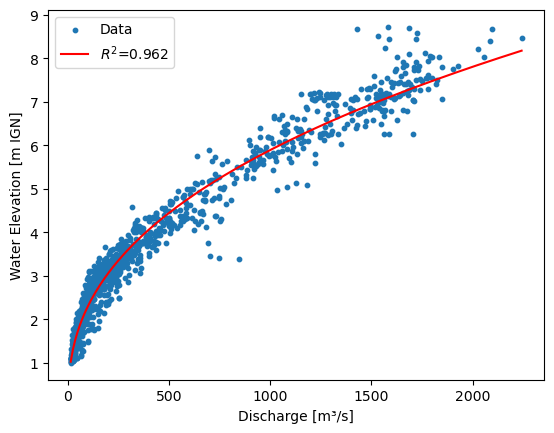
\includegraphics[width=\linewidth]{figures/ch5/wl discharge El Colorado.png}
        \label{fig:water level discharge Colorado}
    \end{subfigure}
    \hfill
    % Second subfigure
    \begin{subfigure}[b]{0.48\linewidth}
        \centering
        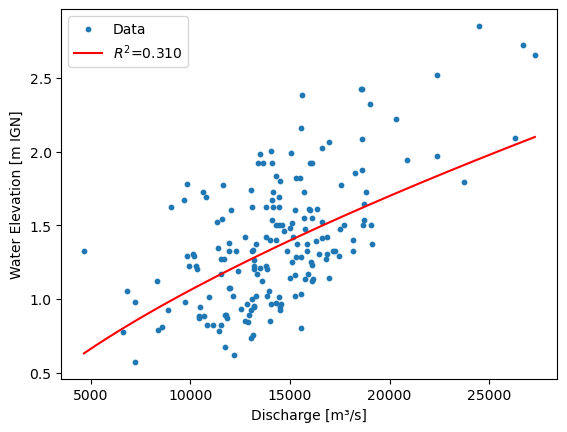
\includegraphics[width=\linewidth]{figures/ch5/wl discharge Brazo Largo.png}
        \label{fig:water level discharge Brazo Largo}
    \end{subfigure}
    \caption{Water elevation - discharge relationship for two measurement stations}
    \label{fig:waterleveldischarge}
\end{figure}



The Paraná Guazu is influenced by both tidal and fluvial controls.
    
- Flow partitioning:
    Gebruik debiet van parana en parana Guazu (zie plot in VScode)
    Gebruik veldwerk metingen om bijdrage rio Ibicuy en rio Talabera te bepalen

\textbf{Flow partitioning}
The Middle Paraná splits 

\begin{figure}[h!]
    \centering
    % First subfigure
    \begin{subfigure}[b]{0.48\linewidth}
        \centering
        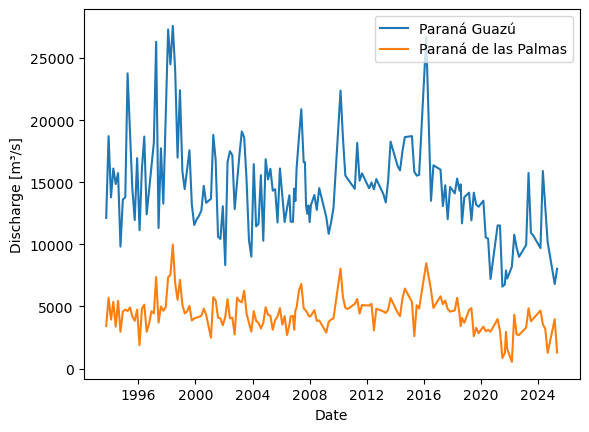
\includegraphics[width=\linewidth]{figures/ch5/discharge series.png}
        \caption{Discharge series obtained from Brazo Largo and Zárate measurement stations}
        \label{fig:discharge_series}
    \end{subfigure}
    \hfill
    % Second subfigure
    \begin{subfigure}[b]{0.48\linewidth}
        \centering
        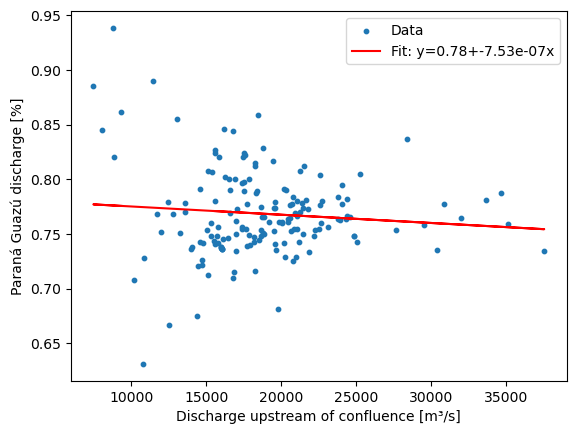
\includegraphics[width=\linewidth]{figures/ch5/flow partition.png}
        \caption{Flow partition, expressed as the share of total flow that streams into Paraná Guazú}
        \label{fig:flow_partition}
    \end{subfigure}
    
    \caption{Comparison between (a) discharge series and (b) flow partition of the Paraná Guazú and Paraná de las Palmas}
\end{figure}



\section{Sediment transport}
From the Brazo Largo measurements, an analysis can be done on the relationship between sediment concentrations and the discharge of the river. Again, a distinction can be made between fine and course sediments. Overall, a power-law fit seems a good approach to model the relation, as shown in Figure \ref{fig:sediments discharge}. The fine sediment concentration is generally higher than the course sediment concentration. In addition, the course sediment concentration increases more significantly for an increasing fluvial discharge. These are general trends, but it has to be stressed that the $R^2$ of both relationships is relatively low. 

\begin{figure}
    \centering
    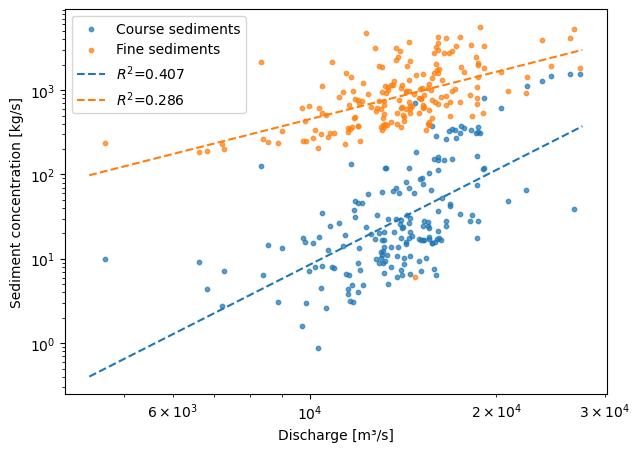
\includegraphics[width=0.5\linewidth]{figures/ch5/Discharge sediment relation.png}
    \caption{Fine and course sediment concentrations in relation to discharge at Brazo Largo}
    \label{fig:sediments discharge}
\end{figure}



- Bepaal fine sediment-discharge relation bij El Colorado. Reken hiermee door voor het fine sediment concentration bij Brazo Largo

- Bepaal fine sediment concentration op basis van de suspended sediment samples.

- Coarse sediment concentration wordt bepaald met de Engelund-Hansen formule

- Vergelijk dit met de bedload metingen van het veldwerk

- Set up a sediment balance for the area of interest.


- Sediment transport caused by tidal assymetry.
% \section{Water Quality and Bioorganism Activity?}


\chapter{Results}
\label{chap:results}
\section{Dredging activities}
This section describes the relevance of dredging to the sediment balance of the designated area, by an estimation of the dredging volumes through different data sources. It includes an analysis of the data gathered through interviews, through AIS data and extraction permits. 

\subsection{Stakeholder interviews}
During the fieldwork, ten interviews with stakeholders were conducted. Responses were recorded and these raw results are given in appendix \ref{chap:interviewres}. The nature of the dredging activities was addressed in almost all interviews. 

\subsubsection{Number of boats}
Stakeholders provided many insights on the scale and development of dredging in the Paraná Guazú river. The caretaker at the Fisher’s Club didn't perceive any increase in recent years, while nearby landowners recalled that the number of dredgers used to be higher, with only two remaining active today. The mayor of Ibicuy confirmed this trend, explaining that most dredging vessels left the Paraná Ibicuy after municipal taxes on sand extraction were raised. At the Port of Ibicuy, the administrator remembered that small dredgers, no longer than twenty meters, once handled sand but have since disappeared; dredging activities there have ceased altogether and moved to a different port (Port Constanza). A private dredger entrepreneur described his own ship, the Vizcaíno 978, which has been prepared for operation after years of administrative delay.

Overall, there is agreement among stakeholders about the number of boats active on the river, namely two. These boats operate in the Paraná Guazú river and not in the Paraná Ibicuy part, since here all dredging activities were stopped.

\subsubsection{Purpose of the sand}
Stakeholders also offered insights into the purposes for which dredged sand is used. According to the the mayor, river sand is generally used for construction materials and, in some cases, glass production. The port administrator confirmed that the sand once handled in Ibicuy was also directed toward the construction sector. The dredger entrepreneur described a mixed market, with sand used primarily for concrete, but also increasingly sold to the fracking industry when sufficiently fine-grained. The YPF mine manager confirmed that the company uses river sand for fracking purposes, although not necessarily from the area of interest.

Overall, stakeholders agreed that construction is the traditional destination of dredged sand. However, multiple stakeholders noted that demand for construction sand has declined in recent years, due to the slowdown of public building projects. In contrast, the demand for fracking sand has been growing steadily, as highlighted by the YPF manager. This shift makes the sale of sand for fracking increasingly viable for producers.

\subsection{Data analysis}
In addition to the stakeholder interview information, AIS data and extraction permits were studied to learn more about the dredging activities on the river. 
\subsubsection{Vessel positioning information (AIS)}
Using MarineTraffic it was found that two dredgers are operating on the Paraná Guazú between Ibicuy and Brazo Largo: the Comercio Segundo and the E.M. Arroyo N1. The Comercio Segundo has a length of 30 m, a width of 7 m, a draft of 1.3 m, and an approximate cargo hold of 195 m\textsuperscript{3}. The E.M. Arroyo N1 has a length of 39 m, a width of 8 m, a draught of 2.8 m and an approximate cargo hold of 476 \,m\textsuperscript{3}. Using a sand to water ratio of 3:1 for the dredged slurry, the amount of sand dredged is 150 \,m\textsuperscript{3} and 360 \,m\textsuperscript{3} respectively per cargo. The tracks of the two vessels obtained from MarineTraffic are shown in Figures 5.1 and 5.2.

\begin{figure}[H]
    \centering
    \begin{minipage}{0.48\textwidth}
        \centering
        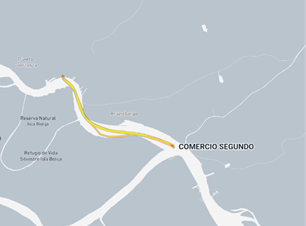
\includegraphics[width=\linewidth]{figures/ch5/Track_CS.png}
        \caption{Track of the \textit{Comercio Segundo}}
        \label{fig:track_cs}
    \end{minipage}\hfill
    \begin{minipage}{0.48\textwidth}
        \centering
        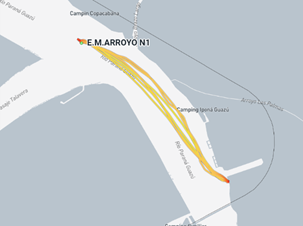
\includegraphics[width=\linewidth]{figures/ch5/Track_EM.png}
        \caption{Track of the \textit{E.M. Arroyo N1}}
        \label{fig:track_em}
    \end{minipage}
\end{figure}

The AIS data for these two vessels is obtained from MyShipTracking, which is used to determine the location of the dredging and the average number of trips. The dredging location of the two vessels is shown in Figure 5.3. It can be seen that both dredgers dredge in the same area. This can be explained by the bathymetry shown in Figure 5.4, which shows a reduced depth near the junction of the two navigable channels. At this location the flow velocity is lower, causing sediment to settle and thus creating a sandbar. From the AIS data it can be concluded that both dredgers make three trips per day.

\begin{figure}[H]
    \centering
    \begin{minipage}{0.48\textwidth}
        \centering
        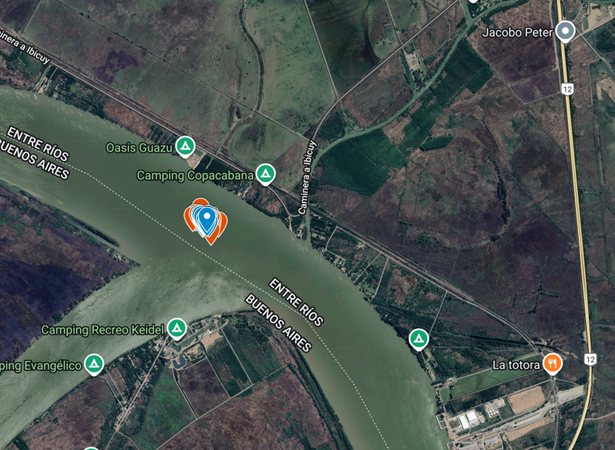
\includegraphics[width=\linewidth]{figures/ch5/Dredging_coordinates.png}
        \caption{Dredging location}
        \label{fig:dredging_coordinates}
    \end{minipage}\hfill
    \begin{minipage}{0.48\textwidth}
        \centering
        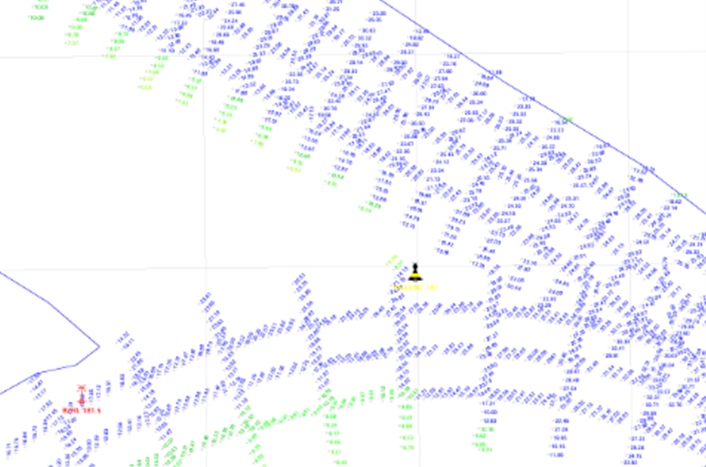
\includegraphics[width=\linewidth]{figures/ch5/Bathymetry.png}
        \caption{Bathymetry}
        \label{fig:bathymetry}
    \end{minipage}
\end{figure}

In the Rio Talabera, a side branch connecting to the Paraná Guazú, a third dredger is extracting sand. The Altair is dredger with a length of 66 m, a width of 11 m, a draught of 1.5 m and a approximate cargo hold of 750 \,m\textsuperscript{3}. Using the same sand to water ratio of 3:1 this gives 560 \,m\textsuperscript{3} of sand per cargo. Using MarineTraffic it was found that the Altair has an average 3 trips per day. Figure 5.5 shows the track of the Altair and the location at which it stops to extract sand. 

\begin{figure}[H]
    \centering
    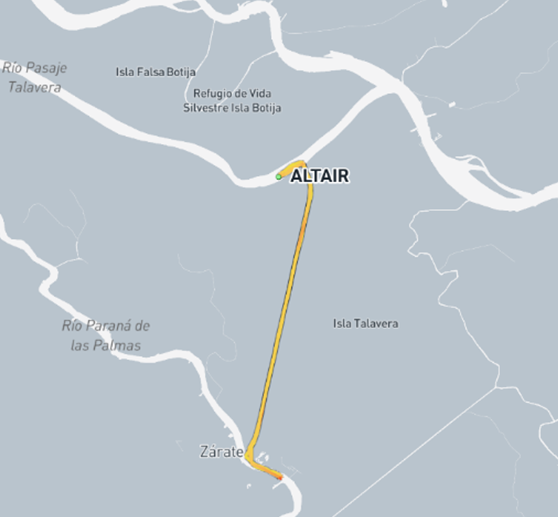
\includegraphics[width=0.5\linewidth]{figures/ch5/Track_Altair.png}
    \caption{Track of the Altair}
    \label{fig:placeholder}
\end{figure}

For all three vessels, the estimated volume of sand extracted per month is displayed in table 5.1
\begin{table}[h!]
\centering
\begin{tabular}{lrrrr}
\hline
\textbf{Vessel} & \textbf{Cargo hold} & \textbf{Sand volume [\,m\textsuperscript{3}]} & \textbf{Trips per day} & \textbf{Volume per month [\,m\textsuperscript{3}]} \\
\hline
Comercio Segundo & 195 & 150 & 3 & 9000 \\
E.M. Arroyo N1 & 476 & 360 & 3 & 21600 \\
Altair & 750 & 560 & 3 & 33600 \\
\hline
\end{tabular}
\caption{Sand transport details per vessel.}
\label{tab:sand_volume}
\end{table}

\subsubsection{Extraction permits}
A total of 33 permits were collected for the Paraná Guazú and 43 for the Ibicuy. On the Paraná Guazú, four permits were issued for channel maintenance, while the remainder concerned sand extraction. For the Ibicuy, all permits were related to extraction activities. The analysis shows that the requested volumes in the Ibicuy are considerably larger than those in the Paraná Guazú, even though the section of the Ibicuy considered here is much shorter in length.

It is important to note that the end dates of contracts are unknown. While the requests specify monthly dredging quantities, they do not indicate the duration of the works. As a result, a detailed quantitative assessment cannot be made. For the present analysis, all requests with fixed monthly volumes are assumed to extend over 12 months, allowing for a comparison between the two river sections, as shown in Figure \ref{fig:yearly dredging volumes}. The second assumption is to record a single value for the requested volume, when information about monthly or yearly occurrence is lacking.

\begin{figure}[H]
    \centering
    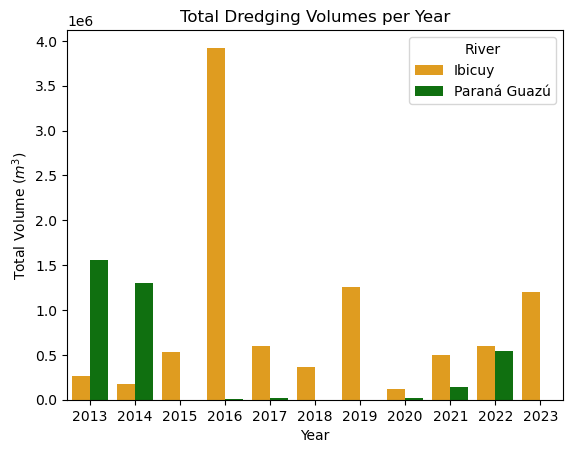
\includegraphics[width=0.50\linewidth]{figures/ch2/Dredging volumes permits.png}
    \caption{Yearly dredging volumes}
    \label{fig:yearly dredging volumes}
\end{figure}

\subsection{Estimated sand extraction}
This section draws a conclusion on the sand extraction volumes, such that an estimate is found to apply in the sediment balance. The following uncertainties were considered in determining a representative value:

\begin{itemize}
    \item Not every vessel in the area is equipped with an AIS transponder, meaning that possibly not all active vessels were identified. However, the number of vessels as found by analysis of the AIS data was in agreement with the number of vessels as observed during the fieldwork.
    \item No historical AIS data was available, such that the data was registered for only a short period of time.
    \item The extraction permits do not mention the duration of the contract.
\end{itemize}

However, a rough estimate can be found by calculating the mean annual volume for the total system of interest (i.e., Ibicuy and Paraná Guazú). To make a comparison with the monthly values in Table \ref{tab:sand_volume}, this yearly value is reduced to a monthly value by dividing by 12 months. The former approach yields the following value for dredged sand volumes:

\begin{equation}
    V_{sand,yearly} = 1193923 ~m^3
\end{equation}
\begin{equation}
    V_{sand,monthly} = \frac{V_{sand,yearly}}{12} \approx 100000 ~m^3 
\end{equation}

\section{Effects of dredging}
This study aims to examine the effects of dredging on the river, with a focus on its ecological and geomorphological impacts. These impacts were explored through a combination of stakeholder interviews and data analysis.

\subsection{Stakeholder interviews}
Stakeholders expressed contrasting views on the ecological and geomorphological impacts of dredging in the Paraná Guazú. Mostly the impacts on fish populations and bank stability were discussed.

\subsubsection{Fish populations}
The caretaker of the Fisher’s Club reported a noticeable decline in fish populations. He did not link this directly to the dredging activities, but instead pointed to contamination from agricultural fertilizers. In contrast, a municipal representative from Zárate questioned the narrative of decline, arguing that complaints about fewer fish reflect generational shifts among fishers rather than an actual reduction.

\subsubsection{Riverbank stability}
When it comes to riverbank stability, landowners described severe erosion of up to thirty metres per year, which they attributed to the activities of dredging vessels and passing cargo ships. The caretaker added that vegetation removal near the club increased local erosion. In contrast to this, the mayor of Ibicuy downplayed the role of dredging, attributing bank collapses in his jurisdiction to the natural flow of the river. Futher, in 2011 there was a qual wall collapse in the Port of Ibicuy, but the portmanager claimed that this was an accident and not due to the sand extraction activities.

\subsection{Data analysis}
Hier hydraulic analyse?
Onderbouwing van wrm baggeren niet zoveel effect heeft

\section{Dry sand mining}


Volumes
Effects
Increase?
Purpose

\subsection{Geological conditions}
Layers
Sand characteristics
\chapter{Mitigation Strategies}


\section{Nature-based Solutions}

When it comes to Nature-based solutions, the question arises what this definition means. A quite general definition of nature based solutions would be;

\textit{“Nature-based Solutions are actions to protect, conserve, restore, sustainably
use and manage natural or modified terrestrial, freshwater, coastal and marine
ecosystems, which address social, economic and environmental challenges
effectively and adaptively, while simultaneously providing human well-being,
ecosystem services, resilience and biodiversity benefits” (United Nations, 2022,
p. 2)}

Although this definition may give a thought that it only concerns natural and biodiversity increasing ideas this is actually not the case. For example the impact of NBS on the local economies and communities is of an equal importance. When it comes to weighing the different NBS against each other this report will make use of the seven goals of the IUCN which must be achieved as good as possible. The seven goals are presented below;

\begin{figure}[H]
    \centering
    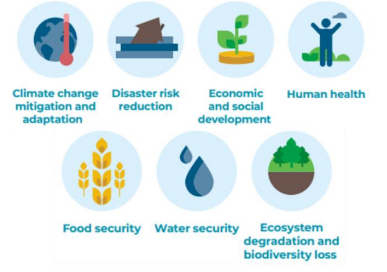
\includegraphics[width=0.50\linewidth]{figures/ThesevenNBSgoals.png}
    \caption{Seven goals for achieving a good NBS}
    \label{fig:placeholder}
\end{figure}

\subsection{Resistance against NBS}

Although NBS are widely known in the scientific world, most people have never heard of these solutions. So, when implementing a solution which can't be described as a classical solution, there is a big change of getting resistance from multiple stakeholders. Especially local communities are skeptical because the solution is less concrete than a classical solution would be. The business case of a NBS must of course also be solid. Without funding of the project, there will never be a change to realize it. That's why it's from great importance to have a solution which is both profitable as explainable to the stakeholders. 

\subsection{Implementing NBS in this project}

As stressed out before in this report, is there a problem with riverbank erosion due to activities on the river. To mitigate or even solve this problem, it is our intend to use a nature based solution. Therefore there are presented multiple possible solutions to create a long-lasting, sustainable riverbank which is made cost effective. These solutions are all graded from one to ten for the seven goals described in section 7.1. The solution which has the highest score will be chosen to mitigate the bank erosion.

One of these solutions is to make a, so said, buffer zone. This means that there is made a swamp area of about 2-8 meter. This gives a change for plants which will hold the soil together. By holding the soil together there will in time be a muddy and organic soil composition, which gives a lot of room for plants and animals to flourish. By doing so, there won't be any erosion on the banks of the river. 


\section{Bed and bank protection measures}

belangrijke/interessante info over deltas en wetlands:
The Paraná Delta, the end of the Paraná-Paraguay river wetland system, begins in the city of Diamante in Entre Ríos province. It stretches for 300 kilometres and covers some 2.3 million hectares. Dotted with islands, these wetlands are a source of ecosystem services such as flood and drought buffering, water purification, erosion control and coastal protection, climate regulation, as well as the provision of shelter, feeding and breeding sites for various wildlife species. It also provides resources including fish, foraging, timber, medicine, and materials for construction and clothing.

In recent years, wetlands have become increasingly important for another key reason: their role as allies against climate change. They improve the resilience of communities to its impacts, serve as natural barriers against floods and droughts, and also function as carbon sinks. Despite playing these important roles, these ecosystems remain under great threat from human action – it is estimated that globally, 85 percent of the wetlands that existed three centuries ago have been destroyed or drastically transformed. 

https://dialogue.earth/en/climate/on-the-parana-river-ecological-crisis-is-a-threat-to-its-identity/


\newpage

\section{Structural Solutions}
There are a number of retaining structures that can be used to stabilize the river banks. Possibilities include:
\begin{itemize}
    \item Sheet pile wall\\
    Sheet pile walls are a common retaining structure and consist of vertical barriers made of interlocking sections. They are a lightweight option and can be removed, which makes them reusable across multiple projects. Another advantage is the fact that installation is relatively easy and therefore cheap. However, sheet pile walls also have limitations. In hard soils and soils with boulders or cobbles, installation becomes difficult. Further, installation can disturb nearby areas through sounds and vibrations. These vibrations can even cause settlements to occur \autocite{mandykorffReaderDeepExcavations2023}.

    \item Diaphragm wall\\
    Diaphragm walls are deep, reinforced concrete retaining structures. They provide excellent structural stability and are capable of resisting significant lateral soil and water pressures. One of their key advantages is water tightness, as they effectively prevent groundwater seepage. They are also suitable for a wide range of soil conditions, and offer durability due to the use of reinforced concrete. On the downside, they are costly to build and require significant time and space due to the specialized equipment, skilled labor, and extensive excavation work that is needed \autocite{mandykorffReaderDeepExcavations2023}.
    
    \item Precast concrete wall\\
    Precast concrete walls are constructed by manufacturing structural elements in a factory environment before transporting them to the construction site. This process allows for superior quality control. Moreover, precast construction can significantly speed up project timelines, as elements are produced in large quantities and quickly installed on-site. Precast concrete offers a long service life with minimal maintenance. Drawbacks of precast concrete walls include: the elements are heavy and thus require specialized transportation and installation equipment \autocite{mcneilengineeringAdvantagesDisadvantagesUsing2023}. Further, the production and transport processes have notable environmental impacts, and repairs or replacements can be complex and costly.

    \item Auger pile wall or soldier pile wall\\
    Auger pile walls and soldier pile walls are widely used in construction for retaining slopes. Auger pile walls are formed by drilling and casting concrete in place, while soldier pile walls consist of vertical steel or timber H-piles with horizontal boards or panels placed between them. They are generally cost-effective solutions that generate minimal vibrations, making them suitable for urban areas and sites sensitive to noise or disturbance. Both systems offer flexibility, allowing adjustments to pile placement, size, and depth to suit specific project requirements. However, leakage between adjacent piles is a relevant risk when it comes to these types of walls \autocite{mandykorffReaderDeepExcavations2023}. Maintaining proper overlap between piles is also critical to ensure structural stability and continuity of the wall.
\end{itemize}

In table \ref{tab:compstruct}, the different structural solutions are summarized and are scored on different relevant criteria.

\begin{table}[H]
\centering
\caption{Comparison of structural solutions}
\resizebox{\textwidth}{!}{%
\begin{tabular}{lcccccccc}
\hline
Method & Installation & Price & Resistance & Versatility & Disturbance & Water tightness & Durability & Sustainability \\
\hline
Sheet pile wall & ++ & + & + & - & - & 0 & + & ++ \\
Diaphragm wall  & -- & -- & ++ & ++ & + & ++ & ++ & - \\
Precast concrete wall & - & - & ++ & 0 & ++ & + & + & -- \\
Auger/Soldier pile wall & + & ++ & 0 & + & ++ & -- & - & 0 \\
\hline
\end{tabular}%
}
\label{tab:compstruct}
\end{table}

As can be seen in table \ref{tab:compstruct}, pile walls score low on water tightness and durability. The area of interest is located in a delta and hence high groundwater levels are to be expected. Therefore, water tightness must be guaranteed. Since the pile walls don't offer this certainty, this option is not further discussed. The diaphragm wall, on the other hand, offers great water tightness but installation is a far bigger challenge for this method. The benefits that the diaphragm wall offers, great resistance and low disturbance being the most relevant ones, do not outweigh the cons: the large amounts of time, space and budget needed to construct them. The same is true for the precast concrete wall: the heavy elements ask for a specialized and expensive installation procedure. The specialized equipment and experience is possibly not available or expensive, which means the precast concrete walls are not a viable option.

As a structural solution, the sheet pile walls are chosen. These elements score high on ease of installation and sustainability (parts can be removed and reused) and price, resistance and durability are also pros of this method. Disturbance is one of the main concerns related to sheet pile walls, but since the area of interest is in a scarcely populated area, this is not necessarily problematic. Another concern is the low versatility: installation is only possible if soils are not too hard. However, since installation will be executed in a delta with relatively soft soil (see xx), this should not be a major concern for this project.

\subsection{Sheet Piles}

Hier bespreken wat sheet piles zijn en in welke situaties we deze kunnen gebruiken. Wellicht een case study bespreken van Pampana waar in een delta achtige rivier dezelfde methode is weten toe te passen.

\subsubsection{Materials}

Hier bespreken van welke materialen deze sheet piles zijn gemaakt in practice.

\subsubsection{Case Study}

Bekijken in de literatuur naar voorbeelden van deze manier van sheet piles in rivieren.

\subsubsection{Cantilever Sheet Piling}

Hier bespreken en laten zien wat cantilever sheet piling is. 

\subsubsection{Failure Mechanisms}

Bespreken wat de mogelijke faal mechanismen zijn van het gerbuik van sheet piles.

\subsubsection{Structural Requirements}

\subsection{Design Methods}

Hier bespreken welke desgin methode we gaan gebruiken. Active en Passive kant van de sheet pile bepalen. Kracht horizontal en momenten som aan nul gelijk stellen om daarmee te bepalen wat de D van de sheet pile moet zijn. Hier een factor overheen gooien. 

\subsection{Design Procedure}

Hier komt de procedure te staan hoe het design tot stand zal gaan komen en welke stappen gemaakt zullen worden.

\subsubsection{Problem Description}

Hier komt een schets van de situatie.

\subsubsection{Geometry of Design}

Hier komt te staan wat de lengte en diepte van de sheet piles zullen worden. En welk profiel gebruikt zal worden voor de sheet piles.

\subsubsection{Internal Loads}

\subsection{Conclusion}


\chapter{Discussion}
\chapter{Stability of the river banks}

Onderzoeken laten zien -> river bank instability
Bepaald wordt -> hoe is het nu en hoe is het in bepaalde gevallen



\section{Geological background}
To understand more about bank erosion, one first must have knowledge of the soil profile in the delta region. This section intends to combine all the available information regarding the subsoil in the investigation area.

\subsection{The geology of a delta}
A delta is a landscape formed at the mouth of a river where the water eventually runs into the ocean. At a delta, the water's velocity decreases which gives floating particles in the delta the change to settle. Among these floating particles are gravels, sands and clays, descending in particle size. The particles are formed by erosion of stone. The origin of the particles in the Parana river are the Andes mountains. 
Besides that, deltas are also characterized by high vegetation growth. When this vegetation dies, the organic material will change into peat due to the governing pressures. So, in a delta one expects to find relatively soft soils (sands) and very soft soils (clay and peat).

\subsection{Geological cross section}
A study by \citeauthor{joseluiscavallottoEvolucionCambiosAmbientales2005} was conducted that led to a morphological map of the Paraná delta. In the study, for two cross sections a more detailed geological profile was made, one of which is relevant to the area of interest. The cross section along with the area of interest is shown in figure \ref{fig:crosssectiongeo}.

\begin{figure}[H]
    \centering
    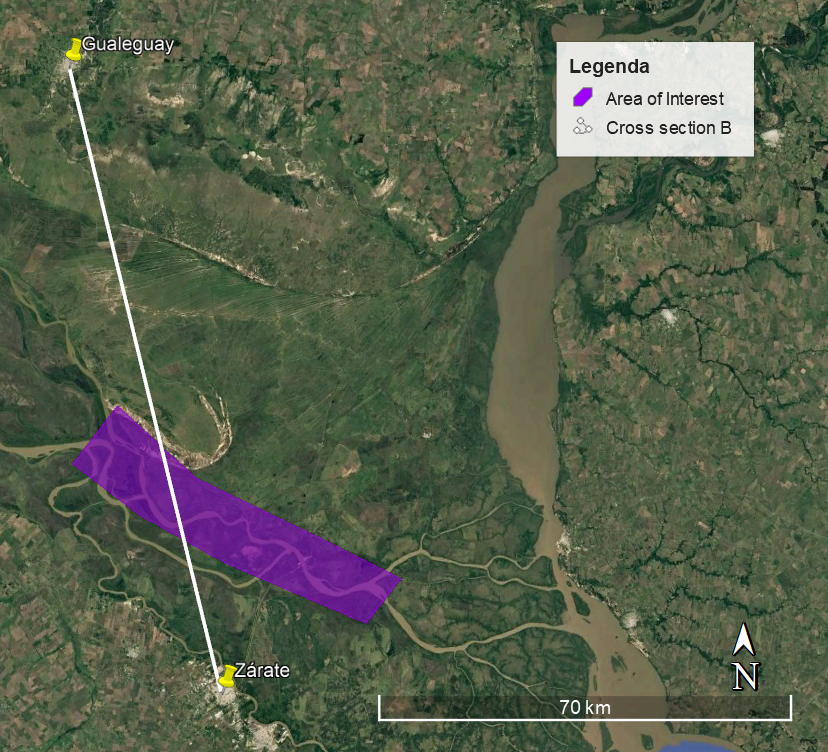
\includegraphics[width=0.75\linewidth]{figures/ch9/CrossSectionB.png}
    \caption{Cross section}
    \label{fig:crosssectiongeo}
\end{figure}

The geological profile of the cross section is shown in figure \ref{fig:geolprofile}. As can be seen in the figure, the taken cross section was around 80 km long. Of this, 15 km falls inside the area of interest, this zone is marked with purple.

\begin{figure}[H]
    \centering
    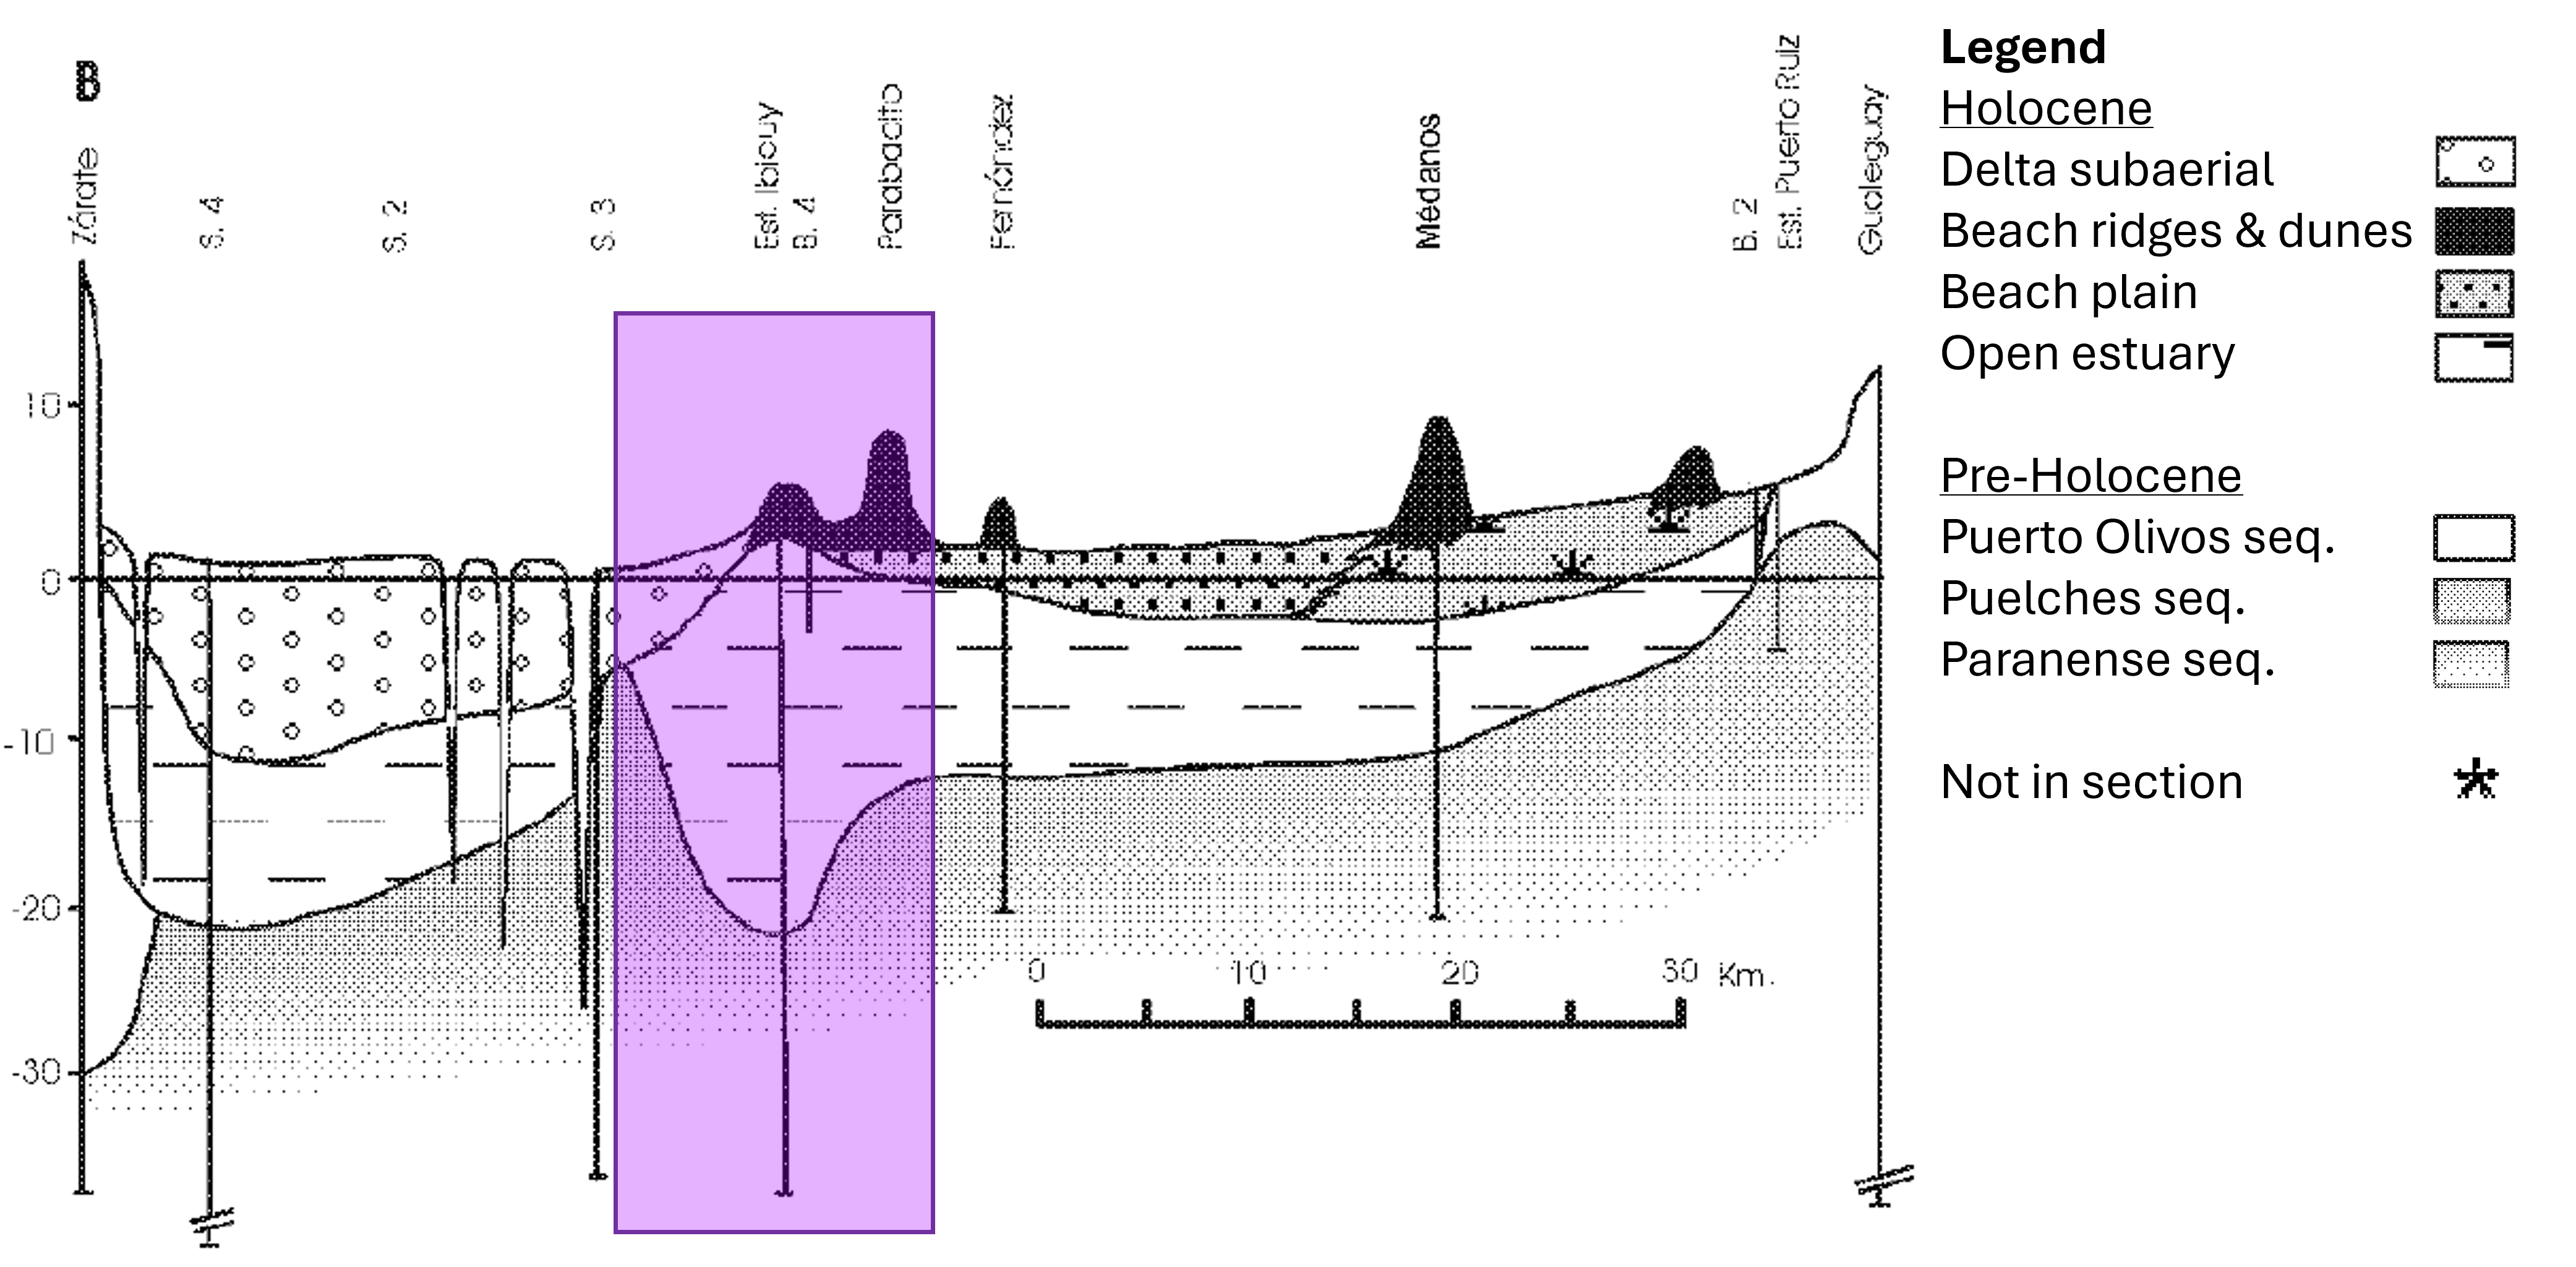
\includegraphics[width=1\linewidth]{figures/ch9/CrossSectionBResults.png}
    \caption{Geological profile of cross section \autocite{joseluiscavallottoEvolucionCambiosAmbientales2005}}
    \label{fig:geolprofile}
\end{figure}

In figure \ref{fig:geolprofile}, the first kilometers of the purple zone are especially of interest since these are located near the river. The following layers can be identified in this area.

\subsubsection{Subaerial facies}
The subaerial facies of the Paraná Delta developed through the deposition of silty-sandy sediments delivered mainly by the Paraná Guazú and Paraná de las Palmas \autocite{joseluiscavallottoEvolucionCambiosAmbientales2005}. These deposits occur at elevations between 2 m and sea level, with a maximum thickness of 12 m. This is the layer that is drained.

Mineralogical analyses show a predominance of quartz with minor plagioclase and K-feldspar, plus heavy minerals such as magnetite, hematite, garnet, zircon, tourmaline, and others, generally well-rounded except zircon, which preserves crystal form \autocite{rafaelcordiniContribucionConocimientoGeologia1949}. The age of the unit is debated: radiocarbon dates suggest origin dates between -150 BC and 180 AD, while other authors propose a later origin around 700–750 AD \autocite{joseluiscavallottoEvolucionCambiosAmbientales2005}.

\subsubsection{Open estuary}
The open estuary sediments were deposited during postglacial sea-level rise and were formed at the freshwater–saltwater interface during the upstream migration of the maximum salinity gradient, which filled the Río de la Plata river valley \autocite{joseluiscavallottoEvolucionCambiosAmbientales2005}.

These are olive-green clays to silty clays with thin fine-sand layers, scattered or concentrated shell beds, and fossil content confirming estuarine conditions. The unit is dated to the Holocene, with its base at ~6670 +/- 100 years BC, occurring between –22 and –0 m and reaching up to 20 m thick \autocite{vogelGroningenRadiocarbonDates1969}.

\subsubsection{Paranense depositional sequence}
During the Miocene, large portions of present-day Argentina, Uruguay, Paraguay, southern Brazil, and eastern Bolivia were covered by the Paranense Sea. This was a shallow sea that advanced from the Atlantic into the interior of South America . Its waters left behind extensive marine sediments and fossils and this layer is now known as the Paranense depositional sequence \autocite{tineoReconstructingSouthAmerican2024}.

It is composed mainly of siliciclastic sandstones, mudstones, and bioclastic beds, with thicknesses ranging from a few meters in outcrop to over 100 m. The lower part has mud-dominated offshore deposits with marine fossils, while the upper part shows sandier shoreface. Studies constrain the unit to the Late Miocene (ca. 9.5–6.7 Ma) \autocite{tineoReconstructingSouthAmerican2024}.

\section{Borehole}
In a different study, a number of boreholes were executed along the lower Paraná.

One of the things that is found about the subsoil is a borehole. This borehole is done in the area of the port of Ibicuy. From this data is made the following soil profile \autocite{amatoESTRATIGRAFIACUATERNARIASUBSUELO2009};

\begin{figure}[H]
    \centering
    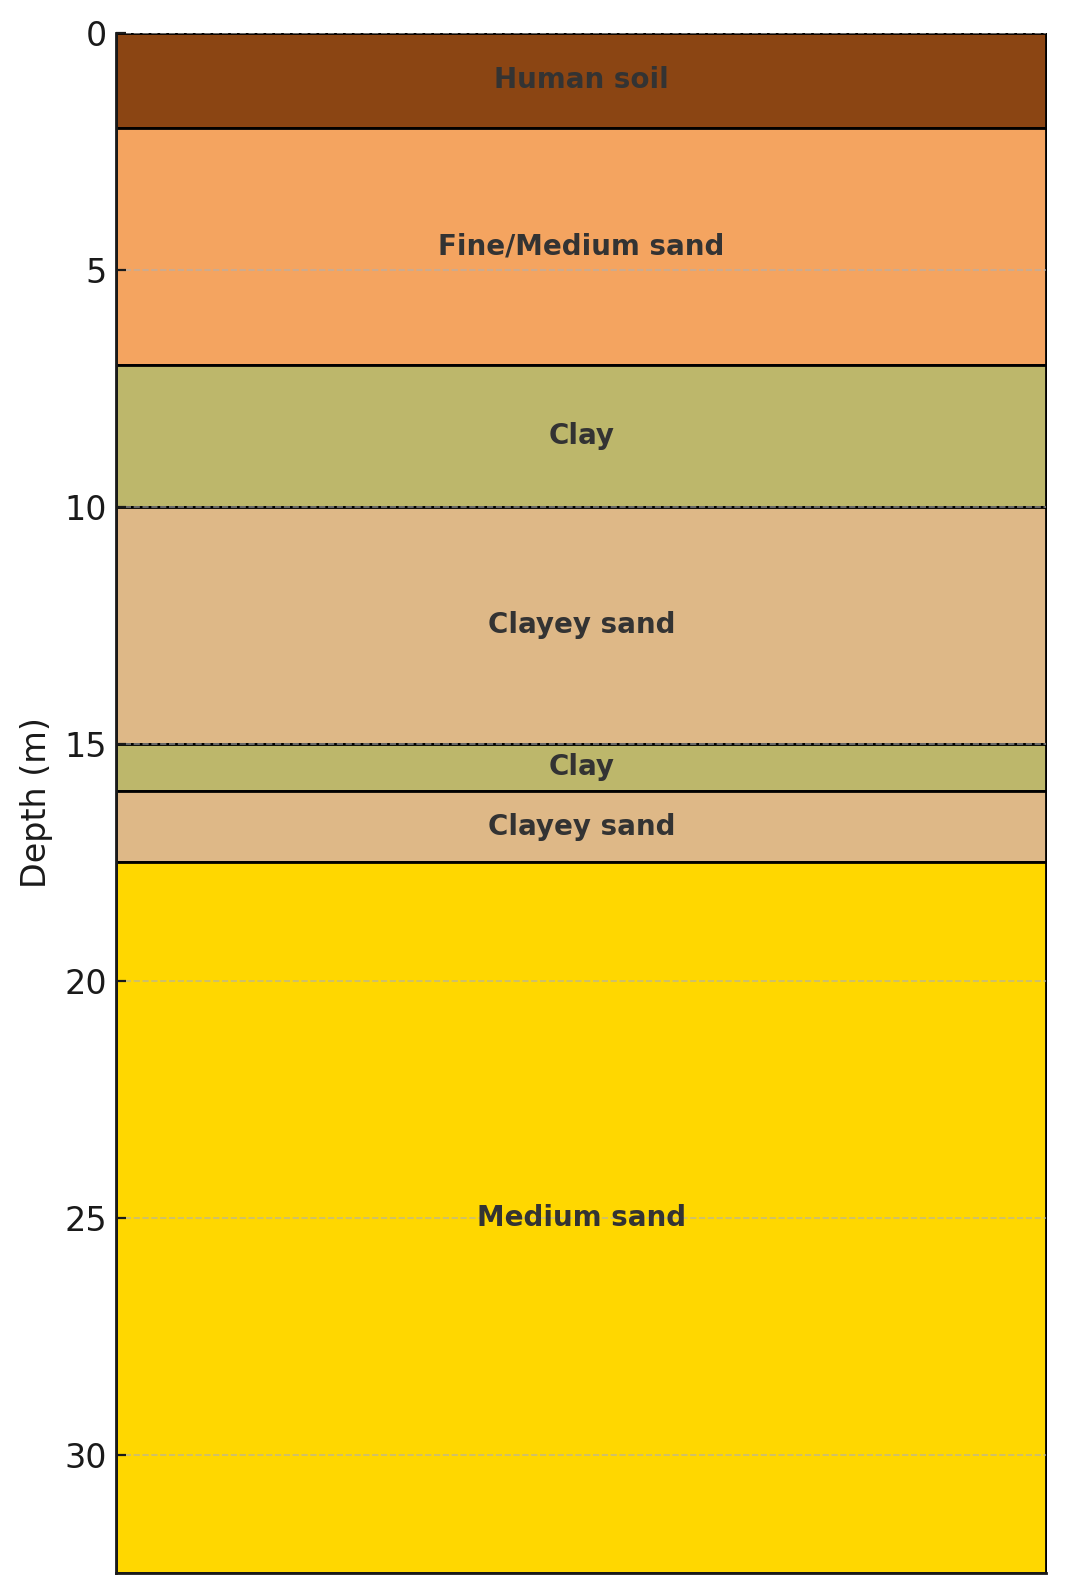
\includegraphics[width=0.45\linewidth]{figures//ch9/Bodemprofiel.png}
    \caption{Borehole profile}
    \label{fig:placeholder}
\end{figure}

\section{Geotechnical summary}
Silty sand

Clay/silty clay

Sandstone/mudstone

\chapter{Conclusion}
\label{chapter:conclusion}

\emph{A conclusion...}


%% Prevent urls running into margins in bibliography
\setcounter{biburlnumpenalty}{7000}
\setcounter{biburllcpenalty}{7000}
\setcounter{biburlucpenalty}{7000}

%% Add bibliography
\printbibliography[heading=bibintoc,title=References]

%% ----------------------------------------------------------------------
%%    Appendix (Letters for chapters)
%% ----------------------------------------------------------------------

\appendix

\chapter{Source Code Example}
%\label{chapter:title}

\emph{Adding source code to your report/thesis is supported with the package {\normalfont\texttt{listings}}. An example can be found below. Files can be added using {\normalfont\texttt{\textbackslash lstinputlisting[language=<language>]\{<filename>\}}}.}

\begin{lstlisting}[language=Python]
"""
ISA Calculator: import the function, specify the height and it will return a
list in the following format: [Temperature,Density,Pressure,Speed of Sound].
Note that there is no check to see if the maximum altitude is reached.
"""

import math
g0 = 9.80665
R = 287.0
layer1 = [0, 288.15, 101325.0]
alt = [0,11000,20000,32000,47000,51000,71000,86000]
a = [-.0065,0,.0010,.0028,0,-.0028,-.0020]

def atmosphere(h):
    for i in range(0,len(alt)-1):
        if h >= alt[i]:
            layer0 = layer1[:]
            layer1[0] = min(h,alt[i+1])
            if a[i] != 0:
                layer1[1] = layer0[1] + a[i]*(layer1[0]-layer0[0])
                layer1[2] = layer0[2] * (layer1[1]/layer0[1])**(-g0/(a[i]*R))
            else:
                layer1[2] = layer0[2]*math.exp((-g0/(R*layer1[1]))*(layer1[0]-layer0[0]))
    return [layer1[1],layer1[2]/(R*layer1[1]),layer1[2],math.sqrt(1.4*R*layer1[1])]
\end{lstlisting}

\chapter{Reflection and Task Division}
\label{chapter:Reflection and Task Division}

\section{Reflection}
Throughout our MDP project, our group maintained a collaborative approach to ensure efficiency and good communication. To optimize our workflow, we divided the team into two groups of three: one attended INA on Mondays, while the other went on Wednesdays. This allowed us to maintain a consistent presence at INA while ensuring all members had equal access to resources and stakeholders. On Tuesdays, the entire group worked at the Boskalis office, creating a productive team alignment since we had access to a blackboard. The remaining days were dedicated to remote work, where we operated as a unified group from home, adhering to a standard internship schedule from 9 to 17, in the living room on the dinner table.


Communication with our supervisors primarily took place during our office days at INA. Outside these days, we relied on digital platforms such as Teams, WhatsApp, and email to stay connected and address any questions or updates. This hybrid approach ensured continuous guidance and support, regardless of our physical location.


Deadlines were managed proactively through a planning process, or spontaneous meetings outside working hours which we developed as a group at the outset of the project. Each milestone and task was discussed collectively, allowing us to give out responsibilities effectively and ensure everyone was aligned with the project’s main question. This approach not only kept us on track but also encouraged open communication and constructive debates during group work sessions.


Overall, the combination of in-person and remote collaboration, clear communication channels, and a well-structured planning process contributed to a productive and cohesive team dynamic. Our ability to adapt to different working environments—whether at INA, Boskalis, or remotely—strengthened our multidisciplinary integration and ensured the successful fulfillment of project requirements.

\section{Task Division}

Throughout the ten weeks of the project every student of the MDP385 Group has actively contributed to the project. 
The contributions have been allocated to one of several students per Chapter in the Report. This can be seen in the Table below.


\begin{table}[H]
    \setlength\extrarowheight{4pt}
    \centering
    \caption{Distribution of the workload}
    \label{tab:taskdivision1}
    \begin{tabularx}{\textwidth}{lXX}
        \toprule
        & Task & Student Name(s) \\
        \midrule
        & Summary & All \\
        Chapter 1 & Introduction & All \\
        \midrule
        Chapter 2 & Background Study & \\
        2.1 & Argentina’s waterways & Victor \\
        2.2 & Classification of Rio Paraná & Victor \\
        2.3 & Origin of sediment content in Paraná Guazú & Jasper \\
        2.4 & Mining of the Sand and Types of Dredging in a River & Niek \\
        2.5 & The effects of river sand mining & Niek \\
        \midrule
        Chapter 3 & Methodology & \\
        3.1 & Data collection & Jasper Stefan\\
        3.2 & Field study & Victor Laurens \\
        3.3 & Setting up the Sediment Balance & Stefan \\
        3.4 & Bank Erosion & Victor \\
        3.5 & Multidisciplinary approach &  Mike \\
        \midrule
        Chapter 4 & Stakeholders & \\
        4.1 & Stakeholder analysis & Mike Niek\\
        4.2 & Interview results & Niek \\
        4.3 & Updated stakeholder analysis & Mike \\
        \midrule
        Chapter 5 & Sand extraction & \\
        5.1 & Dredging activities & Laurens \\
        5.2 & Dry sand mining & Niek Laurens\\
        \midrule
        Chapter 6 & Hydrodynamical and sedimentary analysis & \\
        6.1 & Effect of tides and waves on the water level & Victor\\
        6.2 & Hydrodynamic data & Jasper Stefan\\
        6.3 & Sediment transport & Stefan \\
        6.4 & Field work measurements & Laurens\\
        6.5 & Hydrodynamic effects on the River Banks & Victor \\
        \bottomrule
    \end{tabularx}
\end{table}

\begin{table}[H]
    \setlength\extrarowheight{4pt}
    \centering
    \caption*{}
    \label{tab:taskdivision2}
    \begin{tabularx}{\textwidth}{lXX}
        \toprule
                Chapter 7 & Delft3D Model & Jasper Stefan\\
        \midrule
        Chapter 8 & Mitigation Strategies & \\
        8.1 & Nature-based Solutions for bank erosion & Laurens \\
        8.2 & Structural Solutions for bank erosion & Mike \\
        8.3 & Nature-based Solutions for dry sand mining & Niek \\
        \midrule
        Chapter 9 & Discussion & Niek \\
        \midrule
        Chapter 10 & Conclusion and recommendations & All \\
        \midrule
        Appendix A & Codes?? & Mike \\
        Appendix B & Reflection and Task Division & Victor \\
        Appendix C & Safety Assessment & Laurens \\
        Appendix D & Unprocessed interview results & Niek \\
        Appendix E & Laboratory Data & Victor Laurens \\
        Appendix F & Hydrodynamic Satellite Data & Victor \\
        Appendix G & ADCP Results & Stefan Jasper\\
        \midrule
        & Document Design and Layout & All \\
        \bottomrule
    \end{tabularx}
\end{table}

\section{Fieldwork Tasks and Planning}

For the fieldwork, different tasks were assigned, which were not included in the task division table. 
Therefore, the pdf document used during the trip has been translated and put down below.
Note that repeated info such as list of stakeholders and interview questions have not been included.

\subsubsection{Wednesday (DAY 1)}
8:00 Departure from BA (Group 1 and Group 2)
Group 1: Stefan, Victor, Jasper
Group 2: Niek, Laurens, Mike
Group 1: Boat Group
10:00 Arrive at Recreo Keidel, drop off and set up camping gear, and pay (250,000 ARS).
11:00 Meet the fisherman’s boat with Martin (give money for boat).
11:30 Prepare the boat for Thursday (confirm time, location, and details).
12:30 Prepare equipment and ask for explanations to avoid losing time.
Lunch
Drive to stakeholders (45 min) east of RN12 bridge.
14:30 Camping La Torre
15:30 Yacht Club Guazú
Drive back to camping (30 min)
16:30 Arrive back at camp or similar.
Group 2: Stakeholders (car with marina)
Proposal: Drive directly to Ibicuy to conduct the first interviews and avoid traveling back and forth from the campsite (2.5-hour drive from 9 de Julio Avenue).
Arrive around 10:30–11:00.
Morning interviews if possible, otherwise, schedule after appointments:

Camping Los Abuelos
Camping Boca Del Pavón
Club de Pescadores Olivos (Ibicuy branch)
If time allows, visit the northern end of the area:
Camping El Islerito (above Ibicuy port, quite remote)
Lunch
13:00 Meeting with Ibicuy Port Manager
15:00 Meeting with Ibicuy Mayor
Drive back to camping (1 hour 15 min)
17:00 Arrive back at camp or similar. If earlier, conduct additional interviews around Puerto Guazú.
Ask Marina to translate live if recording is not allowed.


\subsubsection{Thursday (DAY 2)}
Group 1: Stefan, Jasper, Niek
Group 2: Laurens, Mike, Victor
Group 1: Boat Group
Start as early as possible to avoid returning late.
8:00–9:00 Board the boat.
Measurements:

Cross Sections 1, 2, 3 around the dredging point
Discharge measurement with SonTek M9
Flow velocity with radar
Bed load with metal digging tool
Sediment concentration with bottles
Soil sample with excavator
Record notes and trajectory in Locus Map for later GIS import and report inclusion.
Lunch on the boat.
Switch tasks during lunch if possible.
Return to camping by 18:00.

Group 2: Stakeholders
Stay near Guazú for stakeholders; possibly depart at 8:30 (50 min drive to Puerto Guazú).
9:30 Arrive in Puerto Guazú.

9:30 Camping Iponá Guazú
10:00 El Molino Camping
10:30 Port Guazú (Do we have a meeting scheduled, or should we improvise?)
11:00–12:00 Visit Arenera del Guazú to observe small dredging vessels.
Lunch
Drive to Constanza (30 min).
At two small harbors (Constanza and another):
14:00 Camping El Amanecer (near two small harbors)
15:00 Camping La Blanqueada
15:30 Oasis Guazú
Drive back to camping (1 hour).


\subsubsection{Friday (DAY 3)}
Group 1: Laurens, Mike, Victor
Group 2: Jasper, Stefan, Niek
Group 1: Boat Group
8:00–9:00 Board the boat.
1–1:30 Travel to Cross Section 4 in Ibicuy.
Measurements:

Cross Section 4 in Port Ibicuy
Discharge measurement with SonTek M9
Flow velocity with radar
Bed load with metal digging tool
Sediment concentration with bottles
Soil sample with excavator
Record notes and trajectory in Locus Map for later GIS import and report inclusion.
Lunch on the boat.
1–1:30 Travel to Cross Section 4 in Ibicuy.
16:30 Return to camp (estimated by Martin).

Group 2: Stakeholders
9:00 Pack up camping gear and check out.
Reserve day for stakeholders or redistribute tasks, e.g., visit the east side of Puerto Guazú if Group 1 couldn’t on Wednesday. Alternatively, summarize stakeholder findings.
Or:
Drive 45 min east of RN12 bridge.
14:30 Camping La Torre
15:30 Yacht Club Guazú
Drive back to camping (30 min).
Groups 1 and 2:
Drive back to Buenos Aires together, dropping off at strategic locations for faster travel home.
1.5–2 hours drive back to BA.
19:00 Arrive home or similar.

\chapter{Safety assessment}

This appendix presents the risk assessment associated with the procedures that will be conducted in the fieldwork as part of the multiple discipline project titled "Delft University of Technology Sediment Balance in a Sector of the Paraná Guazú River"

\section{Risk Assessment: Fieldwork}

\subsection{Hazard Identification}
This fieldwork involves extensive activities both on and around the water, which inherently present a variety of safety and health hazards. Working in such environments requires continuous awareness and precautionary measures to protect all members of the research team.
The most severe hazard associated with water-based fieldwork is the risk of drowning. This can occur as a result of falling from boats, working on unstable or slippery riverbanks, or being caught in strong currents. Proper use of life jackets, safe boarding procedures, and clear communication within the group are therefore essential preventive measures.

In addition to the immediate risks of drowning, environmental and weather-related factors can also impact safety. High temperatures and prolonged exposure to the sun may cause heat stress, dehydration, or sunburn, while sudden changes in weather—such as heavy rainfall, thunderstorms, or strong winds—can rapidly increase danger on the water. Adequate protective clothing, hydration, and weather monitoring should be part of the fieldwork routine.

Contact with surface water may also expose researchers to biological hazards. Natural water bodies can contain bacteria, parasites, or other microorganisms that cause skin infections or gastrointestinal illness. Wearing waterproof gloves, avoiding direct contact with open wounds, and practicing proper hygiene (e.g., hand washing or use of disinfectants after fieldwork) are effective ways to reduce these risks.
Another aspect to consider is the safe handling of mechanical and sampling equipment. Working with pumps, sieves, augers, or motorized boats requires attention to mechanical hazards such as entanglement, cuts, or equipment malfunction. Ensuring that all equipment is well maintained and operated only by trained individuals minimizes these dangers.

Finally, the natural environment itself may present additional threats from wildlife. These can range from sharp shells or stinging organisms in the water, to insect bites, snakes, or other animals encountered near the riverbank. Using appropriate footwear, insect repellent, and maintaining awareness of the surroundings can help prevent injuries or allergic reactions.


\subsection{Risk Assessment}
The risks associated with this fieldwork vary both in their likelihood of occurrence and in the severity of their potential consequences. Understanding this balance is essential for prioritizing safety measures and ensuring that all critical hazards receive appropriate attention and control.

The risk of drowning, although assessed as having a low likelihood under normal operating conditions, carries extremely severe consequences should it occur. Because of the potentially fatal outcome, this hazard remains a critical concern and must always be treated with the highest level of precaution. Preventive actions such as the mandatory use of life jackets, maintaining clear safety protocols during boat operations, and ensuring all participants are trained in emergency procedures are therefore non-negotiable components of field safety.

Risks arising from weather conditions are more likely to occur and can vary throughout the day. The likelihood of exposure to heat, sun, or sudden changes in weather is considered relatively high, while the potential consequences—ranging from mild heat stress to temporary work interruptions—are moderate. Nevertheless, such risks should be actively mitigated through measures including weather monitoring, adequate rest and hydration, the use of sun protection, and flexible planning to avoid dangerous conditions.

Biological hazards, such as exposure to bacteria or other pathogens present in the water, are generally considered to have a low likelihood of occurrence if proper hygiene and protective measures are followed. However, the consequences of such exposure can be significant, including illness or infection. For this reason, it is vital that all team members remain aware of these hazards and adhere strictly to personal protection and sanitation guidelines, such as using gloves, avoiding contact with open wounds, and washing hands thoroughly after field activities.

Finally, hazards related to mechanical equipment—such as cuts, entanglement, or mechanical malfunction—are assessed as having a low likelihood in this specific fieldwork setting. Their potential consequences are moderate, primarily involving minor injuries or temporary disruption of operations. Routine maintenance, proper training, and adherence to safe operating procedures are sufficient to keep this risk at an acceptable level.


\subsection{Control Measures}
To minimize potential risks during fieldwork, it is essential that all participants make consistent and appropriate use of personal protective equipment (PPE). Key items include life jackets when working on or near the water, sturdy footwear with sufficient grip to prevent slipping on wet or uneven surfaces, and protective gloves when handling tools, equipment, or biological materials. The type of gloves may vary depending on the specific task—ranging from waterproof gloves for wet environments to cut-resistant gloves when working with sharp instruments.

Equally important is ensuring that every team member is fully aware of the hazards present in the field environment. To achieve this, a comprehensive safety briefing must be conducted before any field activities begin. During this briefing, all risks, safety procedures, and emergency response protocols should be clearly explained, allowing participants to understand both their individual responsibilities and the collective safety measures of the group.

Maintaining proper hygiene also plays a crucial role in minimizing biological risks. Regular handwashing, particularly before eating or after contact with river water, significantly reduces the likelihood of bacterial or parasitic infections. The availability of clean water, disinfectant wipes, or alcohol-based sanitizers should therefore be ensured at all times.

In the event of an emergency, effective communication is vital. All team members must be reachable at short notice to enable rapid coordination and response. For this reason, everyone should carry a charged mobile phone at all times. A clear communication plan—including designated contact persons and emergency numbers—should be established before fieldwork begins.

By combining the proper use of PPE, strong situational awareness, good hygiene practices, and reliable communication systems, the risks associated with water-based fieldwork can be significantly reduced, ensuring a safe and efficient working environment for all participants.

\chapter{Safety assessment}

This appendix presents the risk assessment associated with the procedures that will be conducted in the fieldwork as part of the multiple discipline project titled "Delft University of Technology Sediment Balance in a Sector of the Paraná Guazú River"

\section{Risk Assessment: Fieldwork}

\subsection{Hazard Identification}
This fieldwork includes a lot of work around and on the water. Working around water involves several hazards that may affect the safety and health of people in the group. The most extreme risk is the risk of drowning, for example with falls of the boat, unstable banks or strong water currents. Weather conditions can create additional risks such heat stress due to the sun. Contact with water may also result in biological hazards, such as exposure to bacteria. People may also take caution when using mechanical equipment. Finally there are also risks from wildlife (shells, bites and insects). 

\subsection{Risk Assessment}
Risks vary in likelihood and consequence. The risk of drowning is assessed as low in likelihood but is very high in consequence, this makes it a critical concern. The risk due to weather conditions is in likelihood quite high and the consequence is moderate. This makes it a risk which should be mitigated. Biological hazards are quite low in likelihood but are of high consequence, this is why it's important that every staff member is aware of this risk. Mechanical equipment hazard is in our case low in likelihood and moderate in consequence. 


\subsection{Control Measures}
To minimize risks it is important to use some personal protective equipment (PPE) such as life jackets, good footwear which has enough grip, gloves (depending on the work). Every group member must me aware of the risks, that's why there is a safety breefing before operating the fieldwork. Hygiene measures helps reduce biological risks, that's why it's advisable to wash your hands regularly. If there is any form of emergency it's important that everyone is reachable on short notice. That is why everyone should always carry his phone around. 

\end{document}
